\حصہ{سطح طواف کا رقبہ}
بچپن میں آپ نے دوستوں کے ساتھ مل کر رسی گھماتے ہوئے رسی کے اوپر سے چھلانگیں ضرور لگائی ہوں گی۔ یہ رسی فضا میں پھیر  کر ایک سطح بناتی ہے جس کو \اصطلاح{سطح طواف}\فرہنگ{طواف!سطح}\فرہنگ{سطح!طواف}\حاشیہب{surface of revolution}\فرہنگ{revolution!surface} کہتے ہیں۔ سطح طواف کا رقبہ رسی کی لمبائی اور رسی کے ہر حصے کی جھول پر منحصر ہو گا۔ اس حصہ میں سطح طواف کا رقبہ اور سطح کو پیدا کرنے والی منحنی کی لمبائی اور جھول کے تعلق پر غور کیا جائے گا۔زیادہ پیچیدہ سطحوں پر بعد کے باب میں غور کیا جائے گا۔

\جزوحصہء{بنیادی کلیہ}
فرض کریں ہم غیر منفی تفاعل \عددی{y=f(x),\, a\le x\le b} کو \عددی{x}محور کے گرد گھما کر پیدا سطح طواف کا سطحی رقبہ جاننا چاہتے ہیں۔ ہم \عددی{[a,b]} کی خانہ بندی کر کے نقاط خانہ بندی استعمال کرتے ہوئے ترسیم کو چھوٹے حصوں میں تقسیم کرتے ہیں۔ شکل میں نمائندہ حصہ \عددی{PQ}  اور اس کی پیدا کردہ پٹی دکھائی گئی ہے۔

قوس \عددی{PQ} محور \عددی{x} کے گرد گھومتے ہوئے مخروط سطح پیدا کرتی ہے۔محور \عددی{x} اس مخروط سطح کا محور ہو گا۔ مخروط کے ایسے حصے کو \اصطلاح{مخروط مقطوع}\فرہنگ{مخروط مقطوع}\حاشیہب{frustum}\فرہنگ{frustum} کہتے ہیں۔ مخروط مقطوع کا سطحی رقبہ، {PQ} کی پیدا کردہ پٹی کے رقبہ کا تخمین ہو گا۔

مخروط مقطوع کا سطحی رقبہ \عددی{2\pi} ضرب دونوں سروں کے رداس کا اوسط ضرب ترچھا قد کے برابر ہو گا۔
\begin{align*}
\text{\RL{مخروط مقطوع کا سطحی رقبہ}}=2\pi\cdot \frac{r_1+r_2}{2}\cdot L=\pi(r_1+r_2)L
\end{align*} 
قطع \عددی{PQ} کے پیدا کردہ مخروط مقطوع کے لئے اس سے درج ذیل حاصل ہوتا ہے۔
\begin{align*}
\text{\RL{مخروط مقطوع کا سطحی رقبہ}}=
\pi(f(x_{k-1})+f(x_k))\sqrt{(\Delta x_k)^2+(\Delta y_k)^2}
\end{align*}
پوری سطح طواف کا رقبہ تخمیناً ایسے تمام چھوٹے قطعات کی پیدا کردہ مخروط مقطوع کے سطحی رقبوں کا مجموعہ کے ہو گا۔
\begin{align}\label{مساوات_تکمل_استعمال_سطحی_رقبہ_الف}
\sum_{k=1}^n \pi(f(x_{k-1})+f(x_k))\sqrt{(\Delta x_k)^2+(\Delta y_k)^2}
\end{align}
ہم توقع کرتے ہیں کہ \عددی{[a,b]} کی زیادہ باریک خانہ بندی سے تخمین بہتر ہو گی۔ ہم دکھانا چاہتے ہیں کہ خانہ بندی کا معیار صفر تک پہنچنے سے مساوات \حوالہ{مساوات_تکمل_استعمال_سطحی_رقبہ_الف} میں دیا گیا مجموعہ قابل حل حد دیگا۔ 

یہ دکھانے کی خاطر ہم مساوات \حوالہ{مساوات_تکمل_استعمال_سطحی_رقبہ_الف} کو وقفہ \عددی{[a,b]} پر کسی تفاعل  کا ریمان مجموعہ لکھتے ہیں۔لمبائی قوس کے حصول کی طرح ہم تفرقات کے مسئلہ اوسط قیمت کی طرف دیکھتے ہیں۔

اگر \عددی{f} ہموار ہو تب مسئلہ اوسط قیمت کے تحت \عددی{P} اور \عددی{Q} کے بیچ ایسا نقطہ \عددی{(c_k,f(c_k))} ضرور پایا جائے گا جہاں مماس قطع \عددی{PQ} کے متوازی ہو گا۔اس نقطہ پر درج ذیل ہو گا۔
\begin{align*}
f'(c_k)&=\frac{\Delta y_k}{\Delta x_k}\\
\Delta y_k&=f'(c_k)\Delta x_k
\end{align*} 
مساوات \حوالہ{مساوات_تکمل_استعمال_سطحی_رقبہ_الف} میں درج بالا \عددی{\Delta y_k} پر کرتے ہیں۔
\begin{multline}\label{مساوات_تکمل_استعمال_سطحی_رقبہ_ب}
\sum_{k=1}^n \pi(f(x_{k-1})+f(x_k))\sqrt{(\Delta x_k)^2+(\Delta y_k)^2}\\
=\sum_{k=1}^n\pi(f(x_{k-1})+f(x_k))\sqrt{1+(f'(c_k))^2}\Delta x_k
\end{multline}
اب یہاں ایک بری خبر اور ایک اچھی خبر ہے۔

بری خبر یہ ہے کہ مساوات \حوالہ{مساوات_تکمل_استعمال_سطحی_رقبہ_ب} میں  \عددی{x_{k-1}}، \عددی{x_k} اور \عددی{c_k} ایک دوسرے سے مختلف ہیں اور انہیں ایک دوسرے جیسا کسی صورت نہیں بنایا جا سکتا ہے لہٰذا مساوات \حوالہ{مساوات_تکمل_استعمال_سطحی_رقبہ_ب} میں دیا گیا مجموعہ  ریمان مجموعہ نہیں ہے۔ اچھی خبر یہ ہے کہ اس سے کوئی فرق نہیں پڑتا ہے۔ اعلٰی احصاء کا مسئلہ بلس کہتا ہے کہ وقفہ \عددی{[a,b]} کی خانہ بندی کا معیار صفر تک پہچانے سے مساوات \حوالہ{مساوات_تکمل_استعمال_سطحی_رقبہ_ب} میں دیا گیا مجموعہ درج ذیل کو مرکوز ہو گا
\begin{align*}
\int_a^b2\pi f(x)\sqrt{1+(f'(x))^2}\dif x
\end{align*} 
جو ہم چاہتے ہیں۔یوں  \عددی{a} تا \عددی{b} تفاعل \عددی{f} کی ترسیم کو \عددی{x} محور کے گرد گھمانے سے حاصل سطح طواف کے رقبہ کی تعریف ہم اسی تکمل کو لیتے ہیں۔

\ابتدا{تعریف}\موٹا{محور \عددی{x} کے گرد سطح طواف کے رقبہ کا کلیہ}\\
اگر \عددی{[a,b]} پر تفاعل \عددی{f(x)\ge 0} ہموار ہو تب تفاعل \عددی{y=f(x)} کو \عددی{x} محور کے گرد گھمانے سے حاصل سطح طواف کا رقبہ درج ذیل ہو گا۔
\begin{align}\label{مساوات_تکمل_استعمال_سطحی_رقبہ_پ}                                
S=\int_a^b2\pi y\sqrt{1+\big(\frac{\dif y}{\dif x}\big)^2}\dif x=\int_a^b2\pi f(x)\sqrt{1+(f'(x))^2}\dif x
\end{align}
\انتہا{تعریف}
%=========================

مساوات \حوالہ{مساوات_تکمل_استعمال_سطحی_رقبہ_پ} میں جذر وہی ہے جو پیداکار منحنی کی لمبائی قوس کے کلیہ میں پایا جاتا ہے۔

\ابتدا{مثال}
محور \عددی{x} کے گرد منحنی \عددی{y=2\sqrt{x},\, 1\le x\le 2} گھما کر سطح طواف پیدا کیا جاتا ہے۔اس سطح طواف کا رقبہ تلاش کریں۔

حل:\quad
ہم درج ذیل لیتے ہوئے
\begin{align*}
a&=1,\, b=2,\, y=2\sqrt{x},\, \frac{\dif y}{\dif x}=\frac{1}{\sqrt{2}}\\
\sqrt{1+\big(\frac{\dif y}{\dif x}\big)^2}&=\sqrt{1+\big(\frac{1}{\sqrt{x}}\big)^2}\\
&=\sqrt{1+\frac{1}{x}}=\sqrt{\frac{x+1}{x}}=\frac{\sqrt{x+1}}{\sqrt{x}}
\end{align*}
 مساوات \حوالہ{مساوات_تکمل_استعمال_سطحی_رقبہ_پ} استعمال کرتے ہیں۔
\begin{align*}
S&=\int_1^22\pi \cdot2\sqrt{x}\frac{\sqrt{x+1}}{\sqrt{x}}\dif x=4\pi\int_1^2\sqrt{x+1}\dif x\\
&=\left.4\pi\cdot\frac{2}{3}(x+1)^{3/2}\right]_1^2=\frac{8\pi}{3}(3\sqrt{3}-2\sqrt{2})
\end{align*}

\انتہا{مثال}
%=========================

\جزوحصہء{محور \عددی{y} کے گرد سطح طواف}
محور \عددی{y} کے گرد سطح طواف کے لئے ہم مساوات \حوالہ{مساوات_تکمل_استعمال_سطحی_رقبہ_پ} میں \عددی{x} اور \عددی{y} کی جگہیں تبدیل کرتے  ہیں۔

\موٹا{محور \عددی{y} کے گرد سطح طواف کے رقبہ کا کلیہ}\\
اگر \عددی{[c,d]} پر \عددی{x=g(y)\ge 0} ہموار ہو تب منحنی \عددی{x=g(y)} کو محور \عددی{y} کے گرد گھمانے سے حاصل سطح طواف کا رقبہ درج ذیل ہو گا۔
\begin{align}\label{مساوات_تکمل_استعمال_سطحی_رقبہ_ت}
S=\int_c^d2\pi x\sqrt{1+\big(\frac{\dif x}{\dif y}\big)^2}\dif y=\int_c^d2\pi g(y)\sqrt{1+(g'(y))^2}\dif y
\end{align}

\ابتدا{مثال}
لکیری قطع \عددی{x=1-y,\, 0\le y\le 1} کو  محور \عددی{y} کے گرد گھما کر مخروط حاصل کیا جاتا ہے۔ اس کا رقبہ پہلو تلاش کریں۔

حل:\quad
اس رقبہ کو جیومیٹری سے حاصل کیا جا سکتا ہے۔
\begin{align*}
\text{\RL{رقبہ پہلو}}=\frac{\text{\RL{قاعدے کا محیط}}}{2}\times \text{\RL{ترچھا قد}}=\pi \sqrt{2}
\end{align*}
آئیں درج ذیل لے کر  
\begin{align*}
c&=0,\, d=1,\, x=1-y,\, \frac{\dif x}{\dif y}=-1\\
\sqrt{1+\big(\frac{\dif x}{\dif y}\big)^2}&=\sqrt{1+(-1)^2}=\sqrt{2}
\end{align*}
مساوات \حوالہ{مساوات_تکمل_استعمال_سطحی_رقبہ_ت} سے اس رقبہ کا حاصل کریں۔
\begin{align*}
S&=\int_c^d2\pi x\sqrt{1+\big(\frac{\dif x}{\dif y}\big)^2}\dif y=\int_0^12\pi (1-y)\sqrt{2}\dif y\\
&=2\pi \sqrt{2}\left[y-\frac{y^2}{2}\right]_0^1=2\pi \sqrt{2}\big(1-\frac{1}{2}\big)=\pi \sqrt{2}
\end{align*}
دونوں نتائج ایک جیسے ہیں جیسا کہ ہونا چاہیے۔
\انتہا{مثال}
%========================

\جزوحصہء{مختصر تفریقی روپ}
درج ذیل مساواتوں
\begin{align*}
S=\int_a^b2\pi y\sqrt{1+\big(\frac{\dif y}{\dif x}\big)^2}\dif x\quad \text{اور}
\quad S=\int_c^d2\pi x \sqrt{1+\big(\frac{\dif x}{\dif y}\big)^2}\dif y
\end{align*}
کو عموماً تفریقی لمبائی قوس \عددی{\dif s=\sqrt{\dif x^2+\dif y^2}} کی صورت میں لکھا جاتا ہے:
\begin{align*}
S=\int_a^b2\pi y\dif s\quad \text{اور}\quad S=\int_c^d2\pi x\dif s
\end{align*}
بایاں مساوات میں \عددی{x} محور سے قطع \عددی{\dif s} تک فاصلہ \عددی{y} ہے۔ دایاں مساوات میں \عددی{y} محور سے قطع \عددی{\dif s} کا فاصلہ \عددی{x} ہے۔ان دونوں کلیوں کو
\begin{align*}
S=\int 2\pi(\text{\RL{رداس}})(\text{\RL{چوڑائی پٹی}})= \int 2\pi \rho \dif s
\end{align*}
لکھا جا سکتا ہے جہاں رکن لمبائی قوس \عددی{\dif s} تک محور طواف سے فاصلہ \عددی{\rho} ہے۔

\موٹا{مختصر تفریقی روپ}\\
\begin{align*}
S=\int 2\pi \rho \dif s
\end{align*}
کسی مخصوص مسئلے میں آپ رکن لمبائی قوس \عددی{\dif s} اور رداس \عددی{\rho} کو کسی مشترکہ متغیر کی صورت میں لکھ کر تکمل کے حدود بھی اسی متغیر کی روپ میں مہیا کریں گے۔ 

\ابتدا{مثال}
منحنی \عددی{y=x^3,\, 0\le x\le \tfrac{1}{2}} کو محور \عددی{x} کے گرد گھما کر سطح طواف پیدا کیا جاتا ہے۔ اس کا سطحی رقبہ معلوم کریں۔

حل:\quad
ہم مختصر تفریقی روپ سے شروع کرتے ہیں۔
\begin{align*}
S&=\int 2\pi \rho \dif s\\
&=\int 2\pi y\dif s\\
&=\int 2\pi y\sqrt{\dif x^2+\dif y^2}&&\dif s=\sqrt{\dif x^2+\dif y^2}
\end{align*} 
ہم نے یہاں فیصلہ کرنا ہو گا کہ آیا \عددی{\dif s} کو \عددی{\dif x} یا \عددی{\dif y} کی روپ میں لکھیں۔منحنی کی مساوات \عددی{y=x^3} سے \عددی{\dif y} کو \عددی{\dif x} کی صورت میں لکھنا زیادہ آسان ہے لہٰذا ہم درج ذیل استعمال کریں گے۔
\begin{align*}
y=x^3,\, \dif y=3x^2\dif x,\, \sqrt{\dif x^2+\dif y^2}=\sqrt{\dif x^2+(3x^2\dif x)^2}=\sqrt{1+9x^4}\dif x
\end{align*}
انہیں استعمال کرتے ہوئے تکمل کا متغیر \عددی{x} ہو گا۔
\begin{align*}
S&=\int_{x=0}^{x=1/2}2\pi y\sqrt{\dif x^2+\dif y^2}\\
&=\int_0^{1/2}2\pi x^3\sqrt{1+9x^4}\dif x\\
&=\left.2\pi(\tfrac{1}{36})(\tfrac{2}{3})(1+9x^4)^{3/2}\right]_0^{1/2}\\
&=\tfrac{\pi}{27}[(1+\tfrac{9}{16})^{3/2}-1]\\
&=\tfrac{\pi}{27}[(\tfrac{25}{16})^{3/2}-1]\\
&=\tfrac{\pi}{27}(\tfrac{125}{64}-1)\\
&=\tfrac{61\pi}{1728}
\end{align*}
\انتہا{مثال}
%=====================

\حصہء{سوالات}
\موٹا{سطحی رقبہ کے تکمل}\\
سوال \حوالہ{سوال_تکمل_استعمال_سطحی_الف} تا سوال \حوالہ{سوال_تکمل_استعمال_سطحی_ب} میں درج ذیل اقدام کریں۔
\begin{enumerate}[a.]
\item
دیے گئے منحنی کو دیے گئے محور کے گرد گھما کر سطح طواف حاصل کیا جاتا ہے۔ اس کے سطحی رقبے کا تکمل لکھیں۔
\item
منحنی کو ترسیم کر کے اس کی صورت دیکھیں۔ سطحی رقبہ کو بھی ترسیم کریں۔
\item
کمپیوٹر کی مدد سے اس تکمل کو اعدادی طریقہ سے حل کریں۔  
\end{enumerate}

\ابتدا{سوال}\شناخت{سوال_تکمل_استعمال_سطحی_الف}
$y=\tan x,\quad 0\le x \le \tfrac{\pi}{4};\quad \text{\RL{محور \عددی{x}}}$\\
جواب:\quad
(ا) \عددی{2\pi\int_0^{\pi/4}\tan x\sqrt{1+\sec^4x}\dif x}، (ج) \عددی{\approx 3.84}
\انتہا{سوال}
%====================
\ابتدا{سوال}
$y=x^2,\quad 0\le x \le 2;\quad \text{\RL{محور \عددی{x}}}$
\انتہا{سوال}
%====================
\ابتدا{سوال}
$xy=1,\quad 1\le y \le 2;\quad \text{\RL{محور \عددی{y}}}$\\
جواب:\quad
(ا) \عددی{2\pi\int_1^2\tfrac{1}{y}\sqrt{1+y^{-4}}\dif y}، (ج) \عددی{\approx 5.02}
\انتہا{سوال}
%====================
\ابتدا{سوال}
$x=\sin y,\quad 0\le y\le \pi;\quad \text{\RL{محور \عددی{y}}}$
\انتہا{سوال}
%====================
\ابتدا{سوال}
$x^{1/2}+y^{1/2}= 3,\quad \text{\RL{نقطہ $(4,1)$ سے $(1,4)$ تک}};\quad \text{\RL{محور \عددی{x}}}$\\
جواب:\quad
(ا) \عددی{2\pi\int_0^4(3-\sqrt{x})^2\sqrt{1+(1-3x^{-1/2})^2}\dif x}، (ج) \عددی{\approx 63.37}
\انتہا{سوال}
%====================
\ابتدا{سوال}
$y+2\sqrt{y}=x,\quad 1\le y \le 2;\quad \text{\RL{محور \عددی{y}}}$
\انتہا{سوال}
%====================
\ابتدا{سوال}
$x=\int_0^y\tan t\dif t,\quad 0\le y \le\tfrac{\pi}{3};\quad \text{\RL{محور \عددی{y}}}$\\
جواب:\quad
(ا) \عددی{2\pi\int_0^{\pi/3}(\int_0^y\tan t\dif t)\sec y\dif y}، (ج) \عددی{\approx 2.08}
\انتہا{سوال}
%====================
\ابتدا{سوال}\شناخت{سوال_تکمل_استعمال_سطحی_ب}
$y=\int_1^x\sqrt{t^2-1}\dif t,\quad 1\le x \le\sqrt{5};\quad \text{\RL{محور \عددی{x}}}$
\انتہا{سوال}
%====================
\موٹا{سطحی رقبہ کا حصول}\\
\ابتدا{سوال}
لکیری قطع \عددی{y=\tfrac{x}{2},\, 0\le x\le 4} کو \عددی{x} محور کے گرد گھما کر مخروط پیدا کیا جاتا ہے۔ اس کے پہلو کا رقبہ تکمل سے تلاش کریں۔ جیومیٹری کے کلیہ (پہلو کا رقبہ=\عددی{\tfrac{1}{2}}(محیط قاعدہ)(ترچھا قد)) سے اپنے جواب کی تصدیق کریں۔\\
جواب:\quad
$4\pi \sqrt{5}$
\انتہا{سوال}
%==================
\ابتدا{سوال}
لکیری قطع \عددی{y=\tfrac{x}{2},\, 0\le x\le 4} کو \عددی{y} محور کے گرد گھما کر مخروط پیدا کیا جاتا ہے۔ اس کے پہلو کا رقبہ تکمل سے تلاش کریں۔ جیومیٹری کے کلیہ سے اپنے جواب کی تصدیق کریں۔
\انتہا{سوال}
%======================
\ابتدا{سوال}
لکیری قطع \عددی{y=\tfrac{x}{2}+\tfrac{1}{2},\, 1\le x\le 3} کو \عددی{x} محور کے گرد گھما کر مخروط مقطوع پیدا کیا جاتا ہے۔ اس کے پہلو کا رقبہ تکمل سے تلاش کریں۔ جیومیٹری کے کلیہ (رقبہ مخروط مقطوع=\عددی{\pi}(\عددی{r_1+r_2})(ترچھا قد)) سے اپنے جواب کی تصدیق کریں۔\\
جواب:\quad
$3\pi \sqrt{5}$
\انتہا{سوال}
%======================
\ابتدا{سوال}
لکیری قطع \عددی{y=\tfrac{x}{2}+\tfrac{1}{2},\, 1\le x\le 3} کو \عددی{y} محور کے گرد گھما کر مخروط مقطوع پیدا کیا جاتا ہے۔ اس کے پہلو کا رقبہ تکمل سے تلاش کریں۔ جیومیٹری کے کلیہ (رقبہ مخروط مقطوع=\عددی{\pi}(\عددی{r_1+r_2})(ترچھا قد)) سے اپنے جواب کی تصدیق کریں۔
\انتہا{سوال}
%======================
سوال \حوالہ{سوال_تکمل_استعمال_ترسیم_تکمل_الف} تا سوال \حوالہ{سوال_تکمل_استعمال_ترسیم_تکمل_ب} میں منحنی کو دیے گئے محور کے گرد گھما کر سطح  طواف پیدا کیا جاتا ہے۔ اس سطح کا رقبہ معلوم کریں۔ بہتر ہو گا کہ آپ دیے گئے منحنی کو کمپیوٹر پر ترسیم کر کے منحنی کی صورت سیکھیں۔ 

\ابتدا{سوال}\شناخت{سوال_تکمل_استعمال_ترسیم_تکمل_الف}
$y=\tfrac{x^3}{9},\quad 0\le x\le 2,\quad x\,\text{محور}$\\
جواب:\quad
$\tfrac{98\pi}{81}$
\انتہا{سوال}
%=====================
\ابتدا{سوال}
$y=\sqrt{x},\quad \tfrac{3}{4}\le x\le \tfrac{15}{4},\quad x\,\text{محور}$
\انتہا{سوال}
%=====================
\ابتدا{سوال}
$y=\sqrt{2x-x^2},\quad 0.5\le x\le 1.5,\quad x\,\text{محور}$\\
جواب:\quad
$2\pi$
\انتہا{سوال}
%=====================
\ابتدا{سوال}
$y=\sqrt{x+1},\quad 1\le x\le 5,\quad x\,\text{محور}$
\انتہا{سوال}
%=====================
\ابتدا{سوال}
$x=\tfrac{y^3}{3},\quad 0\le y\le 1,\quad y\,\text{محور}$\\
جواب:\quad
$\tfrac{\pi(\sqrt{8}-1)}{9}$
\انتہا{سوال}
%=====================
\ابتدا{سوال}
$x=\tfrac{1}{3}y^{3/2}-y^{1/2},\quad 1\le y\le 3,\quad y\,\text{محور}$
\انتہا{سوال}
%=====================
\ابتدا{سوال}\شناخت{سوال_تکمل_استعمال_ترسیم_موجود_الف}
$x=2\sqrt{4-y},\quad 0\le y\le \tfrac{15}{4},\quad y\,\text{محور}$ 
\quad
(شکل \حوالہ{شکل_سوال_تکمل_استعمال_ترسیم_موجود_الف})\\
جواب:\quad
$\tfrac{35\pi\sqrt{5}}{3}$
\انتہا{سوال}
%=====================
\begin{figure}
\centering
\begin{minipage}{0.45\textwidth}
\centering
\begin{tikzpicture}[font=\small,scale=0.5,declare function={f(\x)=2*sqrt(4-\x);}]
\pgfmathsetmacro{\ra}{f(1)}
\draw[-latex](-4.25,0)--(5,0)node[right]{$x$};
\draw[-latex](0,-0.2)--(0,4.5)node[above]{$y$};
\draw[thick] plot[domain=0:15/4]({f(\x)},\x);
\draw[] plot[domain=0:15/4]({-f(\x)},\x);
\draw(2,{f(2)})node[right,yshift=1ex]{$x=2\sqrt{4-y}$};
\draw(0,15/4) circle (1cm and 0.25cm);
\draw([shift={(180:4cm and 1cm)}]0,0) arc (180:360:4cm and 1cm);
\draw[dashed]([shift={(0:4cm and 1cm)}]0,0) arc (0:180:4cm and 1cm);
\draw(4,0)node[below right]{$4$};
\draw(1,15/4)node[circ]{}++(0,0.1) to [out=45,in=180]++(0.5,0.5)node[right]{$(1,\tfrac{15}{4})$};
\end{tikzpicture}
\caption{}
\label{شکل_سوال_تکمل_استعمال_ترسیم_موجود_الف}
\end{minipage}\hfill
\begin{minipage}{0.45\textwidth}
\centering
\begin{tikzpicture}[font=\small,scale=2,declare function={f(\x)=sqrt(2*\x-1);}]
\pgfmathsetmacro{\ra}{f(1)}
\draw[-latex](-1.15,0)--(1.25,0)node[right]{$x$};
\draw[-latex](0,-0.2)--(0,1.25)node[above]{$y$};
\draw[thick] plot[domain=5/8:1]({f(\x)},\x);
\draw[] plot[domain=5/8:1]({-f(\x)},\x);
\draw(1/2,0)node[below]{$\tfrac{1}{2}$}--++(0,0.1);
\draw(1,0)node[below]{$1$}--++(0,0.1);
\draw(0,1) circle (1cm and 0.15cm);
\draw([shift={(180:0.5cm and 0.15*0.5 cm)}]0,5/8) arc (180:360:0.5cm and 0.15*0.5 cm);
\draw[dashed]([shift={(0:0.5cm and 0.15*0.5 cm)}]0,5/8) arc (0:180:0.5cm and 0.15*0.5 cm);
\draw({f(0.75)},0.75)node[right]{$x=\sqrt{2y-1}$};
\draw({f(1)},1)node[circ]{}node[above,yshift=0.5ex]{$(1,1)$};
\draw({f(5/8)},5/8)node[circ]{}node[below,yshift=-0.5ex]{$(\tfrac{1}{2},\tfrac{5}{8})$};
\end{tikzpicture}
\caption{}
\label{شکل_سوال_تکمل_استعمال_ترسیم_موجود_ب}
\end{minipage}
\end{figure}
\ابتدا{سوال}\شناخت{سوال_تکمل_استعمال_ترسیم_موجود_ب}
$x=\sqrt{2y-1},\quad \tfrac{5}{8}\le y\le 1,\quad y\,\text{محور}$
\quad
(شکل \حوالہ{شکل_سوال_تکمل_استعمال_ترسیم_موجود_ب})
\انتہا{سوال}
%=====================
\ابتدا{سوال}
$x=\tfrac{y^4}{4}+\tfrac{1}{8y^2},\quad 1\le y\le 2,\quad x\,\text{محور}$
\quad
(اشارہ۔ تکمل میں \عددی{\dif s=\sqrt{\dif x^2+\dif y^2}} کو \عددی{\dif y} کی صورت میں لکھ کر \عددی{S=\int 2\pi y \dif s} میں موزوں حد لیتے ہوئے حل کریں۔)\\
جواب:\quad
$\tfrac{253\pi}{20}$
\انتہا{سوال}
%=====================
\ابتدا{سوال}\شناخت{سوال_تکمل_استعمال_ترسیم_تکمل_ب}
$y=\tfrac{1}{3}(x^2+2)^{3/2},\quad 0\le x\le \sqrt{2},\quad y\,\text{محور}$
\quad
(اشارہ۔ تکمل میں \عددی{\dif s=\sqrt{\dif x^2+\dif y^2}} کو \عددی{\dif x} کی صورت میں لکھ کر \عددی{S=\int 2\pi x \dif s} میں موزوں حد لیتے ہوئے حل کریں۔)
\انتہا{سوال}
%=====================
\ابتدا{سوال}\ترچھا{نئی تعریف کی پرکھ}\\
تفاعل \عددی{y=\sqrt{a^2-x^2},\, -a\le x\le x} کو \عددی{x} محور کے گرد گھمانے سے کروی سطح حاصل ہوتا ہے۔ دکھائیں کہ مساوات \حوالہ{مساوات_تکمل_استعمال_سطحی_رقبہ_پ} سے بھی رداس \عددی{a} کرہ کا سطحی رقبہ \عددی{4\pi a^2} حاصل ہوتا ہے۔
\انتہا{سوال}
%=======================
\ابتدا{سوال}\ترچھا{نئی تعریف کی پرکھ}\\
لکیری قطع \عددی{y=\tfrac{r}{h}x,\, 0\le x\le h} کو \عددی{x} محور کے گرد گھمانے سے مخروط پیدا ہوتا ہے جس کے پہلو کا رقبہ \عددی{\pi r\sqrt{r^2+h^2}} ہوتا ہے جہاں مخروط کا قد \عددی{h} اور اس کے قاعدہ کا رداس \عددی{r} ہے لہٰذا اس کے ترچھا قد \عددی{\sqrt{r^2+h^2}} ہو گا۔ تکمل سے مخروط کے پہلو کا رقبہ دریافت کر کے اس کلیہ کی تصدیق کریں۔ 
\انتہا{سوال}
%=================
\ابتدا{سوال}
   (ا) منحنی \عددی{y=\cos x,\, -\tfrac{\pi}{2}\le x\le \tfrac{\pi}{2}} کو \عددی{x} محور کے گرد گھما کر سطح طواف پیدا ہوتا ہے۔ اس سطح طواف کے رقبہ کا تکمل لکھیں جس کو حل کرنا بعد میں سکھایا جائے گا۔ (ب) اس سطحی رقبے کو اعدادی طریقہ سے دریافت کریں۔\\
جواب:\quad
(ا) \عددی{2\pi\int_{-\pi/2}^{\pi/2}(\cos x)\sqrt{1+\sin^2x}\dif x}، (ب) \عددی{\approx 14.4236}
\انتہا{سوال}
%===============
\ابتدا{سوال}\شناخت{سوال_تکمل_استعمال_دوبارہ_ستارہ_نما}\ترچھا{ستارہ نما کا سطحی رقبہ}\\
ستارہ نما \عددی{x^{2/3}+y^{2/3}=1} کا وہ حصہ جو \عددی{x} محور سے اوپر پایا جاتا ہے کو \عددی{x} محور کے گرد گھما کر سطح طواف پیدا کیا جاتا ہے (شکل \حوالہ{شکل_سوال_تکمل_استعمال_دوبارہ_ستارہ_نما})۔ اس سطح طواف کا رقبہ معلوم کریں۔ (اشارہ۔ ربع اول میں منحنی کے حصہ \عددی{y=(1-x^{2/3})^{3/2},\, 0\le x\le 1}) کو \عددی{x} محور کے گرد گھما کر نتیجہ  کو دگنا کریں۔)
\انتہا{سوال}
%================
\begin{figure}
\centering
\begin{minipage}{0.3\textwidth}
\centering
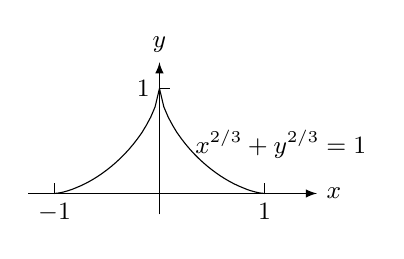
\begin{tikzpicture}[scale=4/3,font=\small,declare function={f(\x)=(1-\x^(2/3))^(3/2);}]
\draw[-latex](-1.25,0)--(1.5,0)node[right]{$x$};
\draw[-latex](0,-0.2)--(0,1.25)node[above]{$y$};
\draw(1,0)node[below]{$1$}--++(0,0.1);
\draw(-1,0)node[below]{$-1$}--++(0,0.1);
\draw(0,1)node[left]{$1$}--++(0.1,0);
\draw[]plot[domain=0:1](\x,{f(\x)});
\draw[]plot[domain=0:1](-\x,{f(\x)});
\draw(0.25,{f(0.25)})node[right]{$x^{2/3}+y^{2/3}=1$};
\end{tikzpicture}
\caption{}
\label{شکل_سوال_تکمل_استعمال_دوبارہ_ستارہ_نما}
\end{minipage}\hfill
\begin{minipage}{0.3\textwidth}
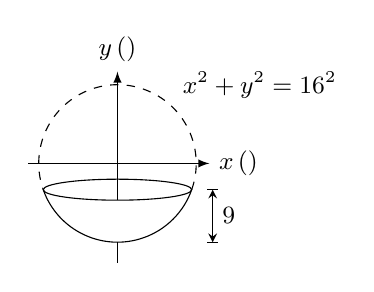
\begin{tikzpicture}[scale=2/3,font=\small]
\centering
\pgfmathsetmacro{\rr}{1.5}
\pgfmathsetmacro{\h}{2*\rr/3}
\pgfmathsetmacro{\r}{sqrt(2*\rr*\h-\h^2)}
\pgfmathsetmacro{\ang}{90-asin(\r/\rr)}
\draw[-latex](-\rr-0.2,0)--(\rr+0.25,0)node[right]{$x\,(\si{\centi\meter})$};
\draw(0,-\rr)--(0,-\rr-0.4);
\draw[-latex](0,-\rr+\h-0.2)--(0,\rr+0.25)node[above]{$y\,(\si{\centi\meter})$};
\draw[dashed]([shift={(-\ang:\rr)}]0,0) arc (-\ang:180+\ang:\rr);
\draw(0,-\rr+\h) circle (\r cm and 0.2 cm);
\draw([shift={(180+\ang:\rr)}]0,0) arc (180+\ang:360-\ang:\rr);
\draw(45:\rr)node[above right]{$x^2+y^2=16^2$};
\draw[stealth-stealth](\r+0.4,-\rr+\h)--++(0,-\h)node[pos=0.5,right]{$\SI{9}{\centi\meter}$};
\draw(\r+0.3,-\rr+\h)--++(0.2,0);
\draw(\r+0.3,-\rr)--++(0.2,0);
\end{tikzpicture}
\caption{}
\label{شکل_سوال_تکمل_استعمال_رنگ}
\end{minipage}\hfill
\begin{minipage}{0.3\textwidth}
\begin{tikzpicture}[scale=1,font=\small,declare function={f(\x)=sqrt(1-\x^2);}]
\pgfmathsetmacro{\k}{0.3}
\pgfmathsetmacro{\t}{0.3}
\draw[-latex](-1.25,0)--(1.5,0)node[right]{$x$};
\draw[-latex](0,-0.2)--(0,1.5)node[above]{$y$};
\draw[-stealth]([shift={(-40:0.2cm and 0.25cm)}]1.4,0) arc (-40:230:0.2cm and 0.25cm);
\draw([shift={(0:1)}]0,0) arc (0:180:1);
\draw(-1,0)node[above left]{$-r$} (1,0)node[above right]{$r$};
\draw(-0.1,{f(0.1)})node[left,yshift=1ex]{$y=\sqrt{r^2-x^2}$};
\draw(\k,0)node[below]{$a$}--(\k,{f(\k)})node[above]{$A$};
\draw(\k+\t,0)--(\k+\t,{f(\k+\t)})node[above]{$B$};
\draw(\k+\t,-0.1)--++(0.5,-0.5)node[below]{$a+h$};
\draw(\k,-3ex)--++(0,-0.2)coordinate[pos=0.5](ka);
\draw(\k+\t,-3ex)--++(0,-0.2)coordinate[pos=0.5](kb);
\draw[stealth-](kb)--++(0.2,0);
\draw[stealth-](ka)--++(-0.3,0)node[left]{$h$};
\draw[fill=lgray]plot[domain=\k:\k+\t](\x,{f(\x)})--(\k+\t,0)--(\k,0)--(\k,{f(\k)});
\end{tikzpicture}
\caption{}
\label{شکل_سوال_تکمل_استعمال_ڈبل_روٹی}
\end{minipage}
\end{figure}
\ابتدا{سوال}\شناخت{سوال_تکمل_استعمال_رنگ}\ترچھا{رنگ}\\
ایک برتن کو رداس \عددی{\SI{16}{\centi\meter}} کے کرہ کا حصہ تصور کیا جا سکتا ہے (شکل \حوالہ{شکل_سوال_تکمل_استعمال_رنگ})۔برتن کی گہرائی \عددی{\SI{9}{\centi\meter}} ہے۔برتن کو اندر اور باہر سے رنگ کرنا مطلوب ہے۔ کچے رنگ کی \عددی{\SI{0.5}{\milli\meter}} موٹی تہہ برتن پر چھڑک کر پکائی جاتی ہے۔ پانچ ہزار برتن کے لئے درکار کچے رنگ کا حجم معلوم کریں۔ رنگ کے ضیاع کو نظر انداز کریں۔\\
جواب:\quad
$\SI{452.4}{\liter}$
\انتہا{سوال}
%======================
\ابتدا{سوال}\شناخت{سوال_تکمل_استعمال_ڈبل_روٹی}\ترچھا{ڈبل روٹی کا کرارا حصہ}\\
ڈبل روٹی اندر سے نرم اور باہر سے کرارا ہوتی ہے۔کیا آپ جانتے ہیں کہ کروی ڈبل روٹی کے ایک جتنی موٹے ٹکڑوں میں  ایک جتنا کرارا حصہ پایا جاتا ہے (شکل \حوالہ{شکل_سوال_تکمل_استعمال_ڈبل_روٹی})؟ یہ دیکھنے کی خاطر نصف دائرہ \عددی{y=\sqrt{r^2-x^2}} کو \عددی{x} محور کے گرد گھما کر کرہ بنائیں۔فرض کریں محور \عددی{x} پر وقفہ \عددی{h} کے اوپر نصف دائرے کا قوس \عددی{AB} ہے۔ دکھائیں کہ نصف دائرے کو \عددی{x} محور کے گرد گھمانے سے \عددی{AB} سے حاصل رقبہ  کی قیمت \عددی{h} کے مقام پر منحصر نہیں ہے۔ (کرارا رقبہ کی قیمت \عددی{h} پر منحصر ہو گی۔)
\انتہا{سوال}
%==================
\ابتدا{سوال}\شناخت{سوال_تکمل_استعمال_کرہ_سے_پٹی}
دو متوازی سطحیں جن کے مابین فاصلہ \عددی{h} ہے رداس \عددی{R} کے کروی سطح سے ایک پٹی کاٹتے ہیں (شکل \حوالہ{شکل_سوال_تکمل_استعمال_کرہ_سے_پٹی})۔ دکھائیں کہ اس پٹی کا رقبہ \عددی{2\pi Rh} ہو گا۔   
\انتہا{سوال}
%===================
\begin{figure}
\centering
\begin{minipage}{0.45\textwidth}
\centering
\begin{tikzpicture}[font=\small,]
\pgfmathsetmacro{\rr}{1.25}
\pgfmathsetmacro{\ka}{0.5}
\pgfmathsetmacro{\ra}{sqrt(\rr^2-\ka^2)}
\pgfmathsetmacro{\kb}{0.6}
\pgfmathsetmacro{\rb}{sqrt(\rr^2-\kb^2)}
\draw(0,0) circle (\rr);
\draw[-latex](0,\rr)node[circ]{}--++(0,0.5)node[above]{$y$};
\draw([shift={(180:\ra cm and 1/4*\ra cm)}]0,\ka) arc (180:360:\ra cm and 1/4*\ra cm);
\draw([shift={(180:\rb cm and 1/4*\rb cm)}]0,\kb) arc (180:360:\rb cm and 1/4*\rb cm);
\draw(\ra,\ka)++(0.1,0)--(\ra+0.3,\ka)coordinate[pos=0.5](aa);
\draw(\rb,\kb)++(0.1,0)--(\ra+0.3,\kb)coordinate[pos=0.5](bb)node[above]{$h$};
\draw[stealth-](aa)--++(0,-0.2);
\draw[stealth-](bb)--++(0,0.2);
\draw[-stealth](0,0)node[circ]{}--++(-45:\rr)node[pos=0.6,fill=white]{$R$};
\end{tikzpicture}
\caption{}
\label{شکل_سوال_تکمل_استعمال_کرہ_سے_پٹی}
\end{minipage}\hfill
\end{figure}
\ابتدا{سوال}
موسمیاتی ریڈار کو شکل میں دکھائے گنبد میں رکھا گیا ہے۔گنبد کا بیرونی رقبہ کتنا ہو گا؟ (قاعدہ کو شامل نہ کریں۔)
\انتہا{سوال}
%====================
\ابتدا{سوال}\ترچھا{محور طواف کو قطع کرنے والے منحنیات سے حاصل سطح طواف}\\
وقفہ \عددی{[a,b]} پر تفاعل \عددی{f} کو غیر منفی تصور کرتے ہوئے  مساوات \حوالہ{مساوات_تکمل_استعمال_سطحی_رقبہ_پ} اخذ کی گئی۔ جہاں تفاعل محور طواف کو قطع کرتا ہو وہاں ہم مساوات \حوالہ{مساوات_تکمل_استعمال_سطحی_رقبہ_پ} کی جگہ درج ذیل مطلق قیمت کلیہ استعمال کرتے ہیں۔
\begin{align}\label{مساوات_تکمل_استعمال_سطحی_رقبہ_ٹ}
S=\int 2\pi \rho \dif s=\int 2\pi \abs{f(x)}\dif s
\end{align}
تفاعل \عددی{y=\tfrac{x^3}{9}-\sqrt{3},\, -\sqrt{3}\le x\le \sqrt{3}}  کو محور \عددی{x} کے گرد گھمانے سے حاصل دوہرا مخروط کا سطحی رقبہ مساوات \حوالہ{مساوات_تکمل_استعمال_سطحی_رقبہ_ٹ} استعمال کرتے ہوئے  دریافت کریں۔\\
جواب:\quad
$5\sqrt{2}\pi$
\انتہا{سوال}
%=================
\ابتدا{سوال}
قوس \عددی{y=\tfrac{x^3}{9}-\sqrt{3},\, -\sqrt{3}\le x\le \sqrt{3}} کو محور \عددی{x} کے گرد گھما کر سطح طواف پیدا کیا جاتا ہے۔ مساوات \حوالہ{مساوات_تکمل_استعمال_سطحی_رقبہ_ٹ} میں مطلق کی علامت ہٹا کر سطحی رقبہ تلاش کرنے سے کیا ہو گا؟
\انتہا{سوال}
%====================
\موٹا{اعدادی تکمل}\\
سوال \حوالہ{سوال_تکمل_استعمال_اعدادی_درستگی_الف} تا سوال \حوالہ{سوال_تکمل_استعمال_اعدادی_درستگی_الف} میں محور \عددی{x} کے گرد دیے گئے منحنیات گھمانے سے سطح طواف پیدا ہوں گے۔ ان سطح طواف کے رقبے اعدادی تراکیب سے \عددی{2} اعشاریہ درستگی تک معلوم کریں۔

\ابتدا{سوال}\شناخت{سوال_تکمل_استعمال_اعدادی_درستگی_الف}
$y=\sin x,\quad 0\le x\le \pi$\\
جواب:\quad
$14.4$
\انتہا{سوال}
%=======================
\ابتدا{سوال}
$y=\tfrac{x^2}{4},\quad 0\le x\le 2$
\انتہا{سوال}
%=======================
\ابتدا{سوال}
$y=x+\sin 2x,\quad -\tfrac{2\pi}{3}\le x\le \tfrac{2\pi}{3}$\\
جواب:\quad
$54.9$
\انتہا{سوال}
%=======================
\ابتدا{سوال}
$y=\tfrac{x}{12}\sqrt{36-x^2},\quad 0\le x\le 6$
\انتہا{سوال}
%=======================
\ابتدا{سوال}\ترچھا{سطحی رقبہ کا متبادل کلیہ}\\
فرض کریں \عددی{[a,b]} پر \عددی{f} ہموار ہے۔ وقفہ \عددی{[a,b]} کی خانہ بندی کریں اور \عددی{k} ویں ذیلی وقفہ \عددی{[x_{k-1},x_k]} کے وسطی نقطہ \عددی{m_k=(\tfrac{x_{k-1}+x_k}{2})} پر منحنی کی مماس لکیر بنائیں۔
\begin{enumerate}[a.]
\item
درج ذیل دکھائیں۔
\begin{align*}
r_1=f(m_k)-f'(m_k)\frac{\Delta x_k}{2},\quad r_2=f(m_k)+f'(m_k)\frac{\Delta x_k}{2}
\end{align*}
\item
دکھائیں کہ \عددی{k} ویں ذیلی وقفہ میں مماسی قطع کی لمبائی \عددی{ L_k=\sqrt{(\Delta x_k)^2+(f'(m_k)\Delta x_k)^2}} ہے۔
\item
دکھائیں کہ مماسی قطع کو محور \عددی{x} کے گرد گھمانے سے حاصل سطح طواف کا رقبہ پہلو \عددی{2\pi f(m_k)\sqrt{1+(f'(m_k))^2}\Delta x_k} ہو گا۔
\item
دکھائیں کہ وقفہ \عددی{[a,b]} پر \عددی{y=f(x)} کو محور \عددی{x} گھمانے سے حاصل سطح طواف کا رقبہ درج ذیل ہو گا۔
\begin{align*}
\lim_{n\to \infty}\sum_{k=1}^n(\text{\RL{$k$ ویں مخروط مقطوع کا رقبہ پہلو}})=\int_a^b2\pi f(x)\sqrt{1+(f'(x))^2}\dif x
\end{align*}
\end{enumerate}
\انتہا{سوال}
%=======================

\حصہ{معیار اثر اور مرکز کمیت}
بہت سارے ساخت اور میکانی نظام کا رویہ ایسا ہوتا ہے جیسا ان کی کمیت ایک نقطہ میں سموئی   ہو جس کو مرکز کمیت کہتے ہیں۔ اس نقطہ کا مقام جاننا اہم ہے جسے ریاضی کی مدد سے معلوم کیا جا سکتا ہے۔ اس باب میں یک بعدی اور دو بعد چیزوں پر توجہ دی جائے گی۔ تین بعدی چیزوں پر بعد کے باب میں غور کیا جائے گا۔

\جزوحصہء{لکیر پر کمیت}
ہم اپنا ریاضی نمونہ بتدریج تیار کرتے ہیں۔ ابتدائی منزل میں ہم  محور \عددی{x} جس کا مبدا اس کا چول ہو، پر کمیت \عددی{m_1}، \عددی{m_2} اور \عددی{m_3} تصور کرتے ہیں۔یہ نظام متوازن یا غیر متوازن ہو گا۔ توازن کا دارومدار کمیتوں کی مقدار اور ان کے مقامات پر منحصر ہے۔ 

\begin{center}
\begin{tikzpicture}
\pgfmathsetmacro{\fa}{0.8}
\pgfmathsetmacro{\fb}{3}
\pgfmathsetmacro{\a}{0}
\pgfmathsetmacro{\b}{1.5}
\pgfmathsetmacro{\c}{5}
\pgfmathsetmacro{\t}{0.25}
\draw[-latex](-0.25,0)--(6.5,0)node[right]{$x$};
\draw(\a,0)node[circ]{}node[below]{$x_1$}node[above]{$m_1$}  (\b,0)node[circ]{}node[below]{$x_2$}node[above]{$m_2$}
   (\c,0)node[circ]{}node[below]{$x_3$}node[above]{$m_3$}; 
\draw[fill=lgray](\fa,0)--++(-\t,-2*\t)--++(2*\t,0)node[pos=0.5,below]{\RL{مبدا پر چول}}--++(-\t,2*\t); 
\end{tikzpicture}
\end{center}
ہر کمیت \عددی{m_k} پر نیچے رخ قوت \عددی{m_kg} عمل کرتا ہے جہاں \عددی{g} ثقلی اسراع ہے (قوت \عددی{m_kg} کو کمیت \عددی{k_k} کا وزن کہتے ہیں)۔ہر ایسی قوت محور کو مبدا کے گرد گھمانے کی کوشش کرتی ہے۔ گھومنے کے اس اثر کو \اصطلاح{قوت مروڑ}\فرہنگ{قوت مروڑ}\حاشیہب{torque}\فرہنگ{torque} کہتے ہیں۔ قوت \عددی{m_kg} کو مبدا سے فاصلہ \عددی{x_k} سے ضرب دینے سے قوت مروڑ کی مقدار حاصل ہوتی ہے جہاں فاصلہ مثبت یا منفی ممکن ہے۔مبدا سے بائیں جانب کمیت منفی (گھڑی مخالف) قوت مروڑ پیدا کرتا ہے جبکہ مبدا سے دائیں جانب کمیت مثبت (گھڑی رخ) قوت مروڑ پیدا کرتا ہے۔

قوت مروڑ کا مجموعہ، مبدا کے گرد نظام گھومنے کے رجحان کا ناپ ہے۔ اس مجموعہ کو \اصطلاح{نظام کی قوت مروڑ}\فرہنگ{قوت مروڑ!نظام}\حاشیہب{system torque}\فرہنگ{torque!system} کہتے ہیں۔
\begin{align}
\text{\RL{نظام کی قوت مروڑ}}=m_1gx_1+m_2gx_2+m_3gx_3
\end{align}
نظام صرف اور صرف اس صورت متوازن ہو گا جب نظام کی قوت مروڑ صفر ہو۔

نظام کی قوت مروڑ کو
\begin{align*}
\underbrace{g}_{\text{\RL{خاصیت ماحول}}}\underbrace{(m_1x_1+m_2x_2+m_3x_3)}_{\text{\RL{خاصیت نظام}}}
\end{align*}
لکھا جا سکتا ہے جہاں \عددی{g} اس ماحول کی خاصیت ہے جس میں نظام پایا جاتا ہے جبکہ  عدد \عددی{(m_1x_1+m_2x_2+m_3x_3)} نظام کی خاصیت ہے جو ایک مستقل ہے اور نظام کو ایک ماحول سے دوسرے ماحول میں منتقل کرنے سے تبدیل نہیں ہوتا۔

عدد \عددی{(m_1x_1+m_2x_2+m_3x_3)} کو \اصطلاح{مبدا کے لحاظ سے نظام کا معیار اثر} کہتے ہیں جو انفرادی کمیت کے معیار اثر \عددی{m_1x_1}، \عددی{m_2x_2} اور \عددی{m_3x_3} کا مجموعہ ہے۔
\begin{align*}
M_0=\text{\RL{مبدا کے لحاظ سے نظام کا معیار اثر}}=\sum m_kx_k
\end{align*}

ہم نظام کو متوازن بنانے کی خاطر نظام کے چول کا مقام جاننا چاہتے ہیں، یعنی چول کو کس نقطہ \عددی{\bar{x}} پر رکھنے سے نظام کا قوت مروڑ صفر ہو گا۔
\begin{center}
\begin{tikzpicture}
\pgfmathsetmacro{\fa}{0.8}
\pgfmathsetmacro{\fb}{3}
\pgfmathsetmacro{\a}{0}
\pgfmathsetmacro{\b}{1.5}
\pgfmathsetmacro{\c}{5}
\pgfmathsetmacro{\t}{0.25}
\draw[-latex](-0.25,0)--(6.5,0)node[right]{$x$};
\draw(\a,0)node[circ]{}node[below]{$x_1$}node[above]{$m_1$}  (\b,0)node[circ]{}node[below]{$x_2$}node[above]{$m_2$}
   (\c,0)node[circ]{}node[below]{$x_3$}node[above]{$m_3$}; 
\draw[dashed](\fa,0)--++(-\t,-2*\t)--++(2*\t,0)node[pos=0.5,below]{مبدا}--++(-\t,2*\t); 
\draw[fill=lgray](\fb,0)node[above]{$\bar{x}$}--++(-\t,-2*\t)--++(2*\t,0)node[pos=0.5,below]{\RL{نقطہ توازن}}--++(-\t,2*\t); 
\end{tikzpicture}
\end{center}
اس مخصوص مقام پر چول رکھنے سے ہر کمیت کا قوت مروڑ درج ذیل لکھا جا سکتا ہے جہاں فاصلہ مثبت یا منفی ہو سکتا ہے۔
\begin{align*}
\text{\RL{$\bar{x}$کے لحاظ سے $m_k$ کا معیار اثر}}&=(\text{\RL{$\bar{x}$ سے $m_k$ کا فاصلہ}})(\text{\RL{نیچے رخ قوت}})\\
&=(x_k-\bar{x})m_kg
\end{align*} 
ان معیار اثر کے مجموعہ کو صفر کے برابر پر کرنے سے ہمیں ایسی مساوات ملتی ہے جسے ہم \عددی{\bar{x}} کے لئے حل کر سکتے ہیں:
\begin{align*}
\sum(x_k-\bar{x})m_kg&=0&&\text{\RL{معیار اثر کا مجموعہ صفر ہے}}\\
g\sum(x_k-\bar{x})m_k&=0&&\text{\RL{مجموعہ کا قاعدہ مستقل مضرب}}\\
\sum(m_kx_k-\bar{x}m_k)&=0&&\text{\RL{$g$ سے تقسیم اور $m_k$ پھیلایا گیا ہے}}\\
\sum m_kx_k-\sum\bar{x}m_k&=0&&\text{\RL{مجموعہ کا قاعدہ فرق}}\\
\sum m_kx_k&=\bar{x}\sum m_k&&\text{\RL{مستقل مضرب قاعدہ اور منتقلی}}\\
\bar{x}&=\frac{\sum m_kx_k}{\sum m_k}&&\text{\RL{$\bar{x}$ کے لئے حل}}
\end{align*} 
یہ آخری مساوات کہتی ہے کہ \عددی{\bar{x}} معلوم کرنے کے لئے مبدا کے لحاظ سے نظام کے معیار اثر کو نظام کی کل کمیت سے تقسیم کریں۔
\begin{align*}
\bar{x}=\frac{\sum x_km_k}{\sum m_k}=\frac{\text{\RL{مبدا کے لحاظ سے نظام کا معیار اثر}}}{\text{\RL{نظام کی کمیت}}}
\end{align*}
نقطہ \عددی{\bar{x}} کو نظام کا \اصطلاح{مرکز کمیت}\فرہنگ{کمیت!مرکز}\حاشیہب{center of mass}\فرہنگ{mass!center of} کہتے ہیں۔

\جزوحصہء{تار اور پتلے سلاخ}
بہت سارے موقعوں پر ہمیں سلاخ یا پتلی پٹی کی کمیت کا مرکز مطلوب ہوتا ہے۔ایسی صورتوں میں اگر ہم تقسیم کمیت  کو استمراری تفاعل کی صورت میں لکھ سکیں  تب ہمارے کلیات میں جمع کی بجائے تکمل ہو گا جیسے نیچے سمجھایا گیا ہے۔

فرض کریں ایک لمبی پٹی \عددی{x=a} تا \عددی{x=b} محور \عددی{x} پر پڑی ہے۔ ہم \عددی{[a,b]} اس پٹی کی خانہ بندی کرتے ہوئے اس کو \عددی{\Delta m_k} کمیت کے چھوٹے چھوٹے  ٹکڑوں میں تقسیم کرتے ہیں۔ \عددی{k} ویں ٹکڑے کی لمبائی \عددی{\Delta x_k} ہے اور یہ مبدا سے تقریباً \عددی{x_k} فاصلے پر پایا جاتا ہے۔اب تین چیزوں کا مشاہدہ کریں۔

\begin{center}
\begin{tikzpicture}[font=\small]
\pgfmathsetmacro{\l}{4.25}
\pgfmathsetmacro{\t}{0.2}
\pgfmathsetmacro{\k}{2.5}
\draw(0,-\t) rectangle (\l,\t);
\draw(-0.1,0)--++(-0.5,0);
\draw[-latex](\l+0.1,0)--++(0.5,0)node[right]{$x$};
\draw[fill=lgray](\k,-\t) rectangle (\k+0.5,\t);
\draw(0,-\t)node[below]{$a$} (\l,-\t)node[below]{$b$};
\draw(\k+0.25,-\t)node[below]{$x_k$};
\draw(\k+0.25,\t)node[above]{$\Delta m_k$};
\draw(\k,-\t-4ex)--++(0,-0.2)coordinate[pos=0.5](ka);
\draw(\k+0.5,-\t-4ex)--++(0,-0.2)coordinate[pos=0.5](kb);
\draw[stealth-](ka)--++(-0.5,0);
\draw[stealth-](kb)--++(0.5,0)--++(0,-0.2)node[below]{$\Delta x_k$};
\end{tikzpicture}
\end{center}
اول، پٹی کا مرکز کمیت \عددی{\bar{x}} اور نقطہ \عددی{x_k} پر کمیت \عددی{\Delta m_k} رکھنے سے حاصل نظام کا مرکز کمیت  تقریباً ایک ہی مقام پر ہوں گے:
\begin{align*}
\bar{x}\approx \frac{\text{\RL{نظام کا معیار اثر}}}{\text{\RL{نظام کی کمیت}}}
\end{align*}

دوم، مبدا کے لحاظ سے ہر ٹکڑے کا معیار اثر تخمیناً \عددی{x_k\Delta m_k} ہو گا لہٰذا نظام کا معیار اثر تخمیناً تمام \عددی{x_k\Delta m_m} کا مجموعہ ہو گا:
\begin{align*}
\text{\RL{نظام کا معیار اثر}}\approx\sum x_k\Delta m_k
\end{align*}

سوم،  اگر \عددی{x_k} پر پٹی کی کثافت \عددی{\delta(x_k)} ہو جہاں \عددی{\delta} استمراری ہے (اور کثافت کی پیمائش کمیت فی لمبائی ہے)  تب \عددی{\Delta m_k} تخمیناً \عددی{\delta(x_k)\Delta x_k} ہو گا:
\begin{align*}
\Delta m_k\approx \delta(x_k)\Delta x_k
\end{align*}

ان تینوں مشاہدوں کو ملا کر درج ذیل حاصل ہو گا۔
\begin{align}\label{مساوات_تکمل_استعمال_مرکز_کمیت_الف}
\bar{x}\approx \frac{\text{\RL{نظام کا معیار اثر}}}{\text{\RL{نظام کی کمیت}}}\approx\frac{\sum x_k\Delta m_k}{\sum \Delta m_k}\approx \frac{\sum x_k\delta(x_k)\Delta x_k}{\sum\delta(x_k)\Delta x_k}
\end{align}
مساوات \حوالہ{مساوات_تکمل_استعمال_مرکز_کمیت_الف} کا آخری شمار کنندہ بند وقفہ \عددی{[a,b]} پر استمراری تفاعل \عددی{x\delta(x)} کا ریمان مجموعہ  ہے جبکہ نسب نما اس وقفہ پر تفاعل \عددی{\delta(x)} کا ریمان مجموعہ ہے۔ہم توقع کرتے ہیں کہ زیادہ باریک خانہ بندی سے مساوات \حوالہ{مساوات_تکمل_استعمال_مرکز_کمیت_الف} میں تخمین بہتر ہوں گے  لہٰذا ہم درج ذیل لکھ سکتے ہیں۔
\begin{align*}
\bar{x}=\frac{\int_a^bx\delta(x)\dif x}{\int_a^b\delta(x)\dif x}
\end{align*} 
ہم \عددی{\bar{x}} کو درج بالا کلیہ سے معلوم کرتے ہیں۔

\موٹا{محور $x$ پر کثافتی تفاعل $\delta(x)$ کے سلاخ یا پٹی کا معیار اثر، کمیت اور مرکز کمیت۔}\\
\begin{gather}
\begin{aligned}\label{مساوات_تکمل_استعمال_مرکز_کمیت_ب}
M_0&=\int_a^bx\delta(x)\dif x&&\text{\RL{مبدا کے لحاظ سے معیار اثر}}\\
M&=\int_a^b\delta(x)\dif x&&\text{\RL{کمیت}}\\
\bar{x}&=\frac{M_0}{M}&&\text{\RL{مرکز کمیت}}
\end{aligned}
\end{gather}

مساوات \حوالہ{مساوات_تکمل_استعمال_مرکز_کمیت_ب} کے حصول میں کثافت کی بات کی گئی۔ عام طور کثافت سے مراد کمیت فی اکائی حجم ہوتا ہے البتہ بعض اوقات ہم وہ اکائیاں استعمال کرتے ہیں جن کی پیمائش نسبتاً زیادہ آسان ہو۔یوں تار، سلاخ اور پٹی کے لئے ہم کمیت فی اکائی لمبائی کو کثافت کہتے ہیں جبکہ مستوی سطحوں کے لئے کمیت فی اکائی رقبہ کو  کثافت کہتے ہیں۔ 

\ابتدا{مثال}\ترچھا{مستقل کثافت کا سلاخ یا پٹی}\\
مستقل کثافت والے سلاخ یا پٹی کا مرکز کمیت تلاش کریں۔

حل:\quad
ہم محور \عددی{x} پر \عددی{x=a} سے \عددی{x=b}  کو سلاخ تصور کرتے ہیں (شکل \حوالہ{شکل_تکمل_استعمال_پتلا_سلاخ})۔ چونکہ کثافت مستقل ہے لہٰذا اس کو تکمل کے باہر منتقل کیا جا سکتا ہے۔یوں درج ذیل حاصل ہوتا ہے۔
\begin{align*}
M_0&=\int_a^b\delta x\dif x=\delta \int_a^bx\dif x=\delta[\frac{x^2}{2}]_a^b=\frac{\delta}{2}(b^2-a^2)\\
M&=\int_a^b\delta \dif x=\delta\int_a^b\dif x=\delta[x]_a^b=\delta(b-a)\\
\bar{x}&=\frac{M_0}{M}=\frac{\frac{\delta}{2}(b^2-a^2)}{\delta (b-a)}=\frac{b+a}{2}
\end{align*}
مستقل کثافت کی صورت میں مرکز کمیت سلاخ یا پٹی کے عین وسطی نقطہ پر ہو گا۔
\انتہا{مثال}
%===============
\begin{figure}
\centering
\begin{minipage}{0.45\textwidth}
\centering
\begin{tikzpicture}[font=\small]
\pgfmathsetmacro{\r}{0.15}
\pgfmathsetmacro{\l}{2.5}
\draw(0,0)circle (1/4*\r cm and \r cm);
\draw(0,\r)--++(\l,0);
\draw(0,-\r)node[below]{$a$}--++(\l,0)node[below]{$b$};
\draw([shift={(-90:1/4*\r cm and \r cm)}]\l,0) arc (-90:90:1/4*\r cm and \r cm);
\draw(-0.1,0)--++(-0.5,0);
\draw[-latex](\l+0.1,0)--++(0.5,0)node[right]{$x$};
\draw(1/2*\l,0)node[circ]{}node[above,yshift=1ex]{\RL{مرکز کمیت}}node[below,yshift=-1ex]{$\tfrac{a+b}{2}$};
\end{tikzpicture}
\caption{مستقل کثافت کے پتلے سیدھے سلاخ کا مرکز کمیت دونوں سروں کے وسطی نقطہ پر ہو گا۔}
\label{شکل_تکمل_استعمال_پتلا_سلاخ}
\end{minipage}\hfill
\begin{minipage}{0.45\textwidth}
\centering
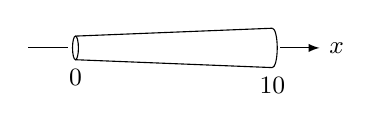
\begin{tikzpicture}[font=\small]
\pgfmathsetmacro{\r}{0.15}
\pgfmathsetmacro{\rr}{0.25}
\pgfmathsetmacro{\l}{2.5}
\draw(0,0)circle (1/4*\r cm and \r cm);
\draw(0,\r)--(\l,\rr);
\draw(0,-\r)node[below]{$0$}--(\l,-\rr)node[below]{$10$};
\draw([shift={(-90:1/4*\rr cm and \rr cm)}]\l,0) arc (-90:90:1/4*\rr cm and \rr cm);
\draw(-0.1,0)--++(-0.5,0);
\draw[-latex](\l+0.1,0)--++(0.5,0)node[right]{$x$};
\end{tikzpicture}
\caption{متغیر موٹائی کے سیدھے سلاخ کو متغیر کثافت کا سیدھا سلاخ تصور کیا جا سکتا ہے۔}
\label{شکل_تکمل_استعمال_متغیر_پتلا_سلاخ}
\end{minipage}
\end{figure}
\ابتدا{مثال}\ترچھا{متغیر کثافت}\\
ایک سلاخ جس کی لمبائی \عددی{\SI{10}{\meter}} ہے بائیں سے دائیں چلتے ہوئے موٹا ہوتا ہے (شکل \حوالہ{شکل_تکمل_استعمال_متغیر_پتلا_سلاخ}) لہٰذا اس کی کثافت مستقل ہونے کی بجائے \عددی{\delta(x)=1+\tfrac{x}{10}\,\si{\kilo\gram\per\meter}} ہے۔ سلاخ کا مرکز کمیت معلوم کریں۔

حل:\quad
ہم مساوات \حوالہ{مساوات_تکمل_استعمال_مرکز_کمیت_ب} استعمال کریں گے۔مبدا کے لحاظ سے سلاخ کا معیار اثر درج ذیل ہو گا۔
\begin{align*}
M_0&=\int_0^{10}x\delta(x)\dif x=\int_0^{10}x\big(1+\frac{x}{10}\big)\dif x
=\int_0^{10}\big(x+\frac{x^2}{10}\big)\dif x\\
&=\big[\frac{x^2}{2}+\frac{x^3}{30}\big]_0^{10}=50+\frac{100}{3}=\frac{250}{3}\,\si{\kilo\gram\meter}
\end{align*}
آپ نے دیکھا کہ معیار اثر کی اکائی \عددی{\si{\kilo\gram\meter}} ہے۔سلاخ کی کمیت درج ذیل ہو گی۔
\begin{align*}
M&=\int_0^{10}\delta(x)\dif x=\int_0^{10}\big(1+\frac{x}{10}\big)\dif x=\big[x+\frac{x^2}{20}\big]_0^{10}10+5=\SI{15}{\kilo\gram}
\end{align*}
مرکز کمیت درج ذیل ہو گا۔
\begin{align*}
\bar{x}=\frac{M_0}{M}=\frac{250}{3}\cdot\frac{1}{15}=\frac{50}{9}\approx \SI{5.56}{\meter}
\end{align*}
\انتہا{مثال}
%======================
\begin{figure}
\centering
\begin{minipage}{0.45\textwidth}
\centering
\begin{tikzpicture}
\draw[-latex](-0.25,0)--(3.5,0)node[right]{$x$};
\draw[-latex](0,-0.2)--(0,2)node[above]{$y$};
\draw(2.5,1.25)node[circ]{}node[above]{$m_k$}node[right,yshift=-1ex]{$(x_k,y_k)$};
\draw(2.5,1.25)--($(0,0)!(2.5,1.25)!(3.5,0)$)coordinate(kB)node[below]{$x_k$}node[pos=0.5,left]{$y_k$};
\draw(2.5,1.25)--($(0,0)!(2.5,1.25)!(0,2)$)coordinate(kL)node[left]{$y_k$}node[pos=0.5,above]{$x_k$};
\RightAngle{(2.5,1.25)}{(kB)}{(0,0)}
\RightAngle{(2.5,1.25)}{(kL)}{(0,0)}
\end{tikzpicture}
\caption{ہر کمیت \عددی{m_k} کا ہر انفرادی محور کے لحاظ سے معیار اثر ہو گا۔}
\label{شکل_تکمل_استعمال_معیار_اثر_تعریف_الف}
\end{minipage}\hfill
\begin{minipage}{0.45\textwidth}
\centering
\begin{tikzpicture}
\draw[-latex](-0.25,0)--(3.5,0)node[right]{$x$};
\draw[-latex](0,-0.2)--(0,2)node[above]{$y$};
\draw(1.75,0)--++(0,2)node[above,align=center]{\RL{لکیر توازن}\\   $x=\bar{x}$};
\draw(0,1)--++(3.5,0)node[right,align=center]{\RL{لکیر توازن}\\ $y=\bar{y}$};
\draw(0.25,0.75)node[circ]{}coordinate(a);
\draw(1,1.75)node[circ]{}coordinate(b);
\draw(2,0.5)node[circ]{}coordinate(c);
\draw(3,1.25)node[circ]{}coordinate(d);
\draw[](a)--($(1.75,0)!(a)!(1.75,2)$);
\draw[](a)--($(0,1)!(a)!(3.5,1)$);
\draw[](b)--($(1.75,0)!(b)!(1.75,2)$);
\draw[](b)--($(0,1)!(b)!(3.5,1)$);
\draw[](c)--($(1.75,0)!(c)!(1.75,2)$);
\draw[](c)--($(0,1)!(c)!(3.5,1)$);
\draw[](d)--($(1.75,0)!(d)!(1.75,2)$);
\draw[](d)--($(0,1)!(d)!(3.5,1)$);
\draw(1.75,1)++(0.05,0.05) to [out=45,in=180]++(0.75,0.75)node[right]{\RL{مرکز کمیت}};
\end{tikzpicture}
\caption{دو بعدی کمیتوں کا جھرمٹ اپنے مرکز کمیت پر متوازن ہو گا۔}
\label{شکل_تکمل_استعمال_معیار_اثر_تعریف_ب}
\end{minipage}
\end{figure}
\جزوحصہء{مستوی پر تقسیم کمیت}
فرض کریں ایک مستوی میں متناہی تعداد میں کمیت پائے جاتے ہیں۔یوں نقطہ \عددی{(x_k,y_k)} پر کمیت \عددی{m_k} ہو گا (شکل \حوالہ{شکل_تکمل_استعمال_معیار_اثر_تعریف_الف})۔اس نظام کی کمیت درج ذیل ہو گی۔
\begin{align*}
M&=\sum m_k&&\text{\RL{نظام کی کمیت}}
\end{align*} 
ہر کمیت \عددی{m_k} کا دونوں محور کے لحاظ سے معیار اثر ہو گا۔ محور \عددی{x} کے لحاظ سے اس کا معیار اثر \عددی{m_ky_k} ہو گا جبکہ محور \عددی{y} کے لحاظ سے  اس کا معیار اثر \عددی{m_kx_k} ہو گا۔دونوں محور کے لحاظ سے پورے نظام کا معیار اثر درج ذیل ہو گا۔
\begin{align*}
M_x&=\sum m_ky_k&&\text{\RL{محور $x$ کے لحاظ سے معیار اثر}}\\
M_y&=\sum m_kx_k&&\text{\RL{محور $y$ کے لحاظ سے معیار اثر}}
\end{align*} 
نظام کے مرکز کمیت کا \عددی{x} محدد درج ذیل ہو گا۔
\begin{align}\label{مساوات_تکمل_استعمال_مرکز_کمیت_ایکس}
\bar{x}=\frac{M_y}{M}=\frac{\sum m_kx_k}{\sum m_k}
\end{align}
یک بعدی صورت کی طرح \عددی{\bar{x}} کی اس قیمت کے لئے نظام لکیر \عددی{x=\bar{x}} پر توازن میں ہو گا (شکل \حوالہ{شکل_تکمل_استعمال_معیار_اثر_تعریف_ب})۔


نظام کے مرکز کمیت کا \عددی{y} محدد درج ذیل ہو گا۔
\begin{align}\label{مساوات_تکمل_استعمال_مرکز_کمیت_وائے}
\bar{y}=\frac{M_x}{M}=\frac{\sum m_ky_k}{\sum m_k}
\end{align}
یک بعدی صورت کی طرح \عددی{\bar{y}} کی اس قیمت کے لئے نظام لکیر \عددی{y=\bar{y}} پر توازن میں ہو گا۔ لکیر \عددی{y=\bar{y}} کے لحاظ سے تمام قوت مروڑ ایک دوسرے کو منسوخ کر کے صفر قوت مروڑ پیدا کرتے ہیں۔ توازن کے اعتبار سے یوں معلوم ہوتا ہے کہ اس نظام کی پوری کمیت نقطہ \عددی{(\bar{x},\bar{y})} میں پائی جاتی ہے۔ اس نقطہ کو نظام کی \اصطلاح{کمیت کا مرکز}\فرہنگ{مرکز!کمیت}\حاشیہب{center of mass}\فرہنگ{mass!center} کہتے ہیں۔

\جزوحصہء{پتلی مستوی چادر}
کئی بار ہمیں پتلی مستوی چادر کا مرکز کمیت درکار ہوتا ہے۔ ایسی صورت میں ہم فرض کرتے ہیں کہ کمیت کی تقسیم استمراری ہے لہٰذا \عددی{\bar{x}} اور \عددی{\bar{y}} کے کلیات میں متناہی مجموعوں کی بجائے تکمل پائے جاتے ہیں۔آئیں اس پر غور کرتے ہیں۔
\begin{figure}
\centering
\begin{tikzpicture}[font=\small]
\pgfmathsetmacro{\k}{1.75}
\pgfmathsetmacro{\kk}{\k+0.2}
\draw[-latex](-0.25,0)--(3,0)node[right]{$x$};
\draw[-latex](0,-0.2)--(0,2)node[above]{$y$};
\path[name path=obj] plot [smooth cycle]coordinates {(0.5,0.5)(1.5,0.7) (2.5,1.5) (2,2) (1,1.5)};
\path[name path=kL](\k,0)--++(0,2.1);
\path[name path=kR](\kk,0)--++(0,2.1);
\draw[name intersections={of=kL and obj,by={a,b}}];
\draw[name intersections={of=kR and obj,by={c,d}}];
\fill[lgray](a)--(b)--(d)--(c)--(a);
\draw(a)--(b)  (c)--(d);
\draw plot [smooth cycle]coordinates {(0.5,0.5)(1.5,0.7) (2.5,1.5) (2,2) (1,1.5)};
\draw($(a)!0.5!(d)$)node[circ]{}node[below left]{$(\tilde{x},\tilde{y})$}++(0.2,0)to[out=0,in=180]++(0.45,-0.25)node[right]{\RL{پٹی کا مرکز کمیت}};
\draw[dashed]($(a)!0.5!(c)$)coordinate(kx)--($(0,0)!(kx)!(2,0)$)node[below]{$\tilde{x}$};
\draw[dashed]($(a)!0.5!(d)$)coordinate(ky)--($(0,0)!(ky)!(0,2)$)node[left]{$\tilde{y}$};
\draw($(b)!0.5!(d)$)++(0,-0.1) to [out=90,in=-90]++(-0.25,0.25)node[above]{\RL{پٹی کی کمیت $\dif m$ ہے}};
\end{tikzpicture}
\caption{چادر کو انتصابی پتلی پٹیوں میں تقسیم کیا گیا ہے۔ نمائندہ پٹی کا کسی ایک انفرادی محور کے لحاظ سے معیار اثر وہی ہو گا جو پٹی کی کمیت \عددی{\dif m} کو پٹی کی مرکز کمیت پر منجمد کرنے سے حاصل ہو گا۔}
\label{شکل_تکمل_استعمال_چادر_انتصابی_پٹی_مرکز_کمیت}
\end{figure}
فرض کریں \عددی{xy} مستوی میں ایک پتلی چادر پائی جاتی ہے۔ چادر کو کسی ایک محور کے متوازی باریک پٹیوں میں تقسیم کریں (شکل \حوالہ{شکل_تکمل_استعمال_چادر_انتصابی_پٹی_مرکز_کمیت} میں پٹیاں محور \عددی{y} کے متوازی ہیں)۔ کسی ایک نمائندہ پٹی کی کمیت کا مرکز \عددی{(\tilde{x},\tilde{y})} ہو گا۔ ہم پٹی کی کمیت \عددی{\Delta m} کو نقطہ \عددی{(\tilde{x},\tilde{y})} پر منجمد تصور کرتے ہیں۔یوں محور \عددی{y} کے لحاظ سے پٹی کا معیار اثر \عددی{\tilde{x}\Delta m} ہو گا جبکہ محور \عددی{x} کے لحاظ سے پٹی کا معیار اثر \عددی{\tilde{y}\Delta m} ہو گا۔ اس طرح مساوات \حوالہ{مساوات_تکمل_استعمال_مرکز_کمیت_ایکس} اور مساوات \حوالہ{مساوات_تکمل_استعمال_مرکز_کمیت_وائے} درج ذیل صورت اختیار کرتے ہیں۔
\begin{align*}
\bar{x}=\frac{M_y}{M}=\frac{\sum \tilde{x}\Delta m}{\sum \Delta m},\quad \bar{y}=\frac{M_x}{M}=\frac{\sum \tilde{y}\Delta m}{\sum \Delta m}
\end{align*}
یک بعدی صورت کی طرح یہاں بھی ریمان مجموعے پائے جاتے ہیں جن کی قیمتیں، پٹی کی چوڑائی کم سے کم کرنے سے قطعی تکملات کی قیمتیں ہوں گی۔ ان تکملات کو علامت طور پر درج ذیل لکھا جاتا ہے۔
\begin{align*}
\bar{x}=\frac{\int \tilde{x}\dif m}{\int \dif m},\quad \bar{y}=\frac{\int\tilde{y}\dif m}{\int\dif m}
\end{align*} 

\موٹا{\عددی{} مستوی میں باریک چادر کے معیار اثر، کمیت اور مرکز کمیت۔}
\begin{gather}
\begin{aligned}
M_x&=\int \tilde{y}\dif m&&\text{\RL{محور $x$ کے لحاظ سے معیار اثر}}\\
M_y&=\int\tilde{x}\dif m&&\text{\RL{محور $y$ کے لحاظ سے معیار اثر}}\\
M&=\int \dif m&&\text{\RL{کمیت}}\\
\bar{x}&=\frac{M_y}{M},\quad \bar{y}=\frac{M_x}{M}&&\text{\RL{مرکز کمیت}}
\end{aligned}
\end{gather}

ان تکملات کی حصول کے لئے ہم چادر کو محددی مستوی میں رکھ کر کسی ایک محدد کے متوازی  ایک نمائندہ پٹی کا خاکہ بناتے ہیں۔ اس پٹی کی کمیت اور مرکز کمیت کے محدد \عددی{ (\tilde{x},\tilde{y})} کو \عددی{x} اور \عددی{y} کی صورت میں لکھا جاتا ہے۔ اس کے بعد محددی مستوی میں چادر کے مقام کے اعتبار سے موزوں حدود کے بیچ  \عددی{\tilde{y}\dif m}، \عددی{\tilde{x}\dif m} اور \عددی{\dif m} کے تکملات  لیتے ہیں۔

\ابتدا{مثال}\شناخت{مثال_تکمل_استعمال_چادر_کثافت}
ایک تکونی چادر جس کو شکل \حوالہ{شکل_مثال_تکمل_استعمال_چادر_کثافت}-ا میں دکھایا گیا ہے کی مستقل کثافت \عددی{\delta =\SI{3}{\gram\per\centi\meter\cubed}} ہے۔ (ا) محور \عددی{y} کے لحاظ سے چادر کا معیار اثر \عددی{M_y} معلوم کریں۔ (ب) چادر کی کمیت \عددی{M} معلوم کریں۔ (ج) چادر کی کمیت کے مرکز کا \عددی{\bar{x}} محدد معلوم کریں۔

حل:\quad
\موٹا{پہلی ترکیب:} \ترچھا{انتصابی پٹیاں} (شکل \حوالہ{شکل_مثال_تکمل_استعمال_چادر_کثافت}-ب)\\
(ا) نمائندہ پٹی کے لئے درج ذیل لکھا جا سکتا ہے۔
\begin{multicols}{2}
\begin{enumerate}[]
\item
مرکز کمیت:\quad
    $(\tilde{x},\tilde{y})=(x,y)$
\item
لمبائی:\quad
$2x$
\item
رقبہ:\quad
$\dif S=2x\dif x$
\item
چوڑائی:\quad
$\dif x$
\item
کمیت:\quad
$\dif m=\delta \dif A=3\cdot2x\dif x=6x\dif x$\\
\item
مرکز کمیت کا محور \عددی{y} سے فاصلہ:\quad
$\tilde{x}=x$
\end{enumerate}
\end{multicols}
یوں محور \عددی{y} کے لحاظ سے پٹی کا معیار اثر
\begin{align*}
\tilde{x}\dif m=x\cdot 6x\dif x=6x^2\dif x
\end{align*}
ہو گا لہٰذا پوری چادر کا محور \عددی{y} کے لحاظ سے معیار اثر درج ذیل ہو گا۔
\begin{align*}
M_y=\int\tilde{x}\dif m=\int_0^1 6x^2\dif x=\left.2x^3\right]_0^1=\SI{2}{\gram\centi\meter}
\end{align*}
(ب) چادر کی کمیت درج ذیل ہو گی۔
\begin{align*}
M=\int \dif m=\int_0^16x\dif x=\left.3x^2\right]_0^1=\SI{3}{\gram}
\end{align*}
(ج) چادر کے مرکز کمیت کا \عددی{x} محدد درج ذیل ہو گا۔
\begin{align*}
\bar{x}=\frac{M_y}{M}=\frac{\SI{2}{\gram\centi\meter}}{\SI{3}{\gram}}=\frac{2}{3},\si{\centi\meter}
\end{align*}
\موٹا{دوسری ترکیب:} \ترچھا{افقی پٹیاں}  (شکل \حوالہ{شکل_مثال_تکمل_استعمال_چادر_کثافت}-ج)\\
(ا) نمائندہ انتصابی پٹی کے مرکز کمیت کا \عددی{y} محدد \عددی{y} ہو گا:
\begin{align*}
\tilde{y}=y
\end{align*}
پٹی کے دائیں اور بائیں سروں کے وسط میں \عددی{x} محدد پایا جائے گا:
\begin{align*}
\tilde{x}=\frac{\frac{y}{2}+1}{2}=\frac{y}{4}+\frac{1}{2}=\frac{y+2}{4}
\end{align*}
اس کے علاوہ درج ذیل بھی لکھا جا سکتا ہے۔
\begin{multicols}{2}
\begin{enumerate}[]
\item
لمبائی:\quad
$1-\frac{y}{2}=\frac{2-y}{2}$
\item
چوڑائی:\quad
$\dif y$
\item
رقبہ:\quad
$\dif S=\frac{2-y}{2}\dif y$
\item
کمیت:\quad
$\dif m=\delta \dif S=3\cdot\frac{2-y}{2}\dif y$
\item
مرکز کمیت کا محور \عددی{y} سے فاصلہ:\quad
$\tilde{x}=\frac{y+2}{4}$
\end{enumerate}
\end{multicols}
یوں محور \عددی{y} کے لحاظ سے پٹی کا معیار اثر
\begin{align*}
\tilde{x}\dif m=\frac{y+2}{4}\cdot 3\cdot \frac{2-y}{2}\dif y=\frac{3}{8}(4-y^2)\dif y
\end{align*}
ہو گا اور محور \عددی{y} کے لحاظ سے چادر کا معیار اثر درج ذیل ہو گا۔
\begin{align*}
M_y=\int\tilde{x}\dif m=\int_0^2\frac{3}{8}(4-y^2)\dif y=\frac{3}{8}\left[4y-\frac{y^3}{3}\right]_0^2=\frac{3}{8}\left(\frac{16}{3}\right)=\SI{2}{\gram\centi\meter}
\end{align*}
(ب) چادر کی کمیت درج ذیل ہو گی۔
\begin{align*}
M=\int\dif m=\int_0^2\frac{3}{2}(2-y)\dif y=\frac{3}{2}\left[2y-\frac{y^2}{2}\right]_0^2=\frac{3}{2}(4-2)=\SI{3}{\gram}
\end{align*}
(ج) چادر کی مرکز کمیت کا \عددی{x} محدد درج ذیل ہو گا۔
\begin{align*}
\bar{x}=\frac{M_y}{M}=\frac{\SI{2}{\gram\centi\meter}}{\SI{3}{\gram}}=\frac{2}{3}\,\si{\centi\meter}
\end{align*}
ہم اسی طرح \عددی{M_x} اور \عددی{\bar{y}} بھی تلاش کر سکتے ہیں۔
\انتہا{مثال}
%=========================
\begin{figure}
\centering
\begin{subfigure}{0.3\textwidth}
\centering
\begin{tikzpicture}[font=\small,xscale=2]
\draw[-latex](-0.25,0)--(1.25,0)node[right]{$x\,(\si{\centi\meter})$};
\draw[-latex](0,-0.2)--(0,2.25)node[above]{$y\,(\si{\centi\meter})$};
\draw[fill=lgray](0,0)--(1,2)node[pos=0.75,above left]{$y=2x$}--(1,0)node[pos=0.5,right]{$x=1$}node[below]{$1$}--(0,0);
\draw(0.5,0)node[below]{$y=0$} (0,2)node[left]{$2$}--++(0.1,0);
\end{tikzpicture}
\caption{تکونی چادر۔}
\end{subfigure}\hfill
\begin{subfigure}{0.3\textwidth}
\centering
\begin{tikzpicture}[font=\small,xscale=2,declare function={f(\x)=2*\x;}]
\pgfmathsetmacro{\k}{0.6}
\pgfmathsetmacro{\t}{0.05}
\draw[-latex](-0.25,0)--(1.25,0)node[right]{$x\,(\si{\centi\meter})$};
\draw[-latex](0,-0.2)--(0,2.25)node[above]{$y\,(\si{\centi\meter})$};
\draw[](0,0)--(1,2)node[pos=0.9,left]{$y=2x$}node[right]{$(1,2)$}--(1,0)node[below]{$1$};
\draw(0,2)node[left]{$2$}--++(0.1,0);
\draw[fill=lgray,opacity=0.5](\k-\t,0)rectangle(\k+\t,{f(\k)});
\draw(\k,{1/2*f(\k)})node[circ]{}node[right,fill=white,xshift=1ex]{$(\tilde{x},\tilde{y})=(x,x)$};
\draw(\k-\t,-0.1)--++(0,-0.2)coordinate[pos=0.7](kL);
\draw(\k+\t,-0.1)--++(0,-0.2)coordinate[pos=0.7](kR);
\draw[stealth-](kL)--++(-0.1,0);
\draw[stealth-](kR)--++(0.1,0)--++(0,-0.1)node[below]{$\dif x$};
\draw(\k,{f(\k)})node[left]{$(x,2x)$};
\draw[stealth-stealth](0,{1/2*f(\k)})--(\k,{1/2*f(\k)})node[pos=0.25,above]{$x$};
\end{tikzpicture}
\caption{انتصابی پٹیاں۔}
\end{subfigure}\hfill
\begin{subfigure}{0.3\textwidth}
\centering
\begin{tikzpicture}[font=\small,xscale=2,declare function={f(\x)=2*\x;}]
\pgfmathsetmacro{\k}{0.6}
\pgfmathsetmacro{\t}{0.05}
\draw[-latex](-0.25,0)--(1.25,0)node[right]{$x\,(\si{\centi\meter})$};
\draw[-latex](0,-0.2)--(0,2.25)node[above]{$y\,(\si{\centi\meter})$};
\draw[](0,0)--(1,2)node[right]{$(1,2)$}--(1,0)node[below]{$1$};
\draw(0,2)node[left]{$2$}--++(0.1,0);
\draw[fill=lgray,opacity=0.5](1,{f(\k-\t)})rectangle(\k,{f(\k+\t)});
\draw({\k+1/2*(1-\k)},{f(\k)})node[circ]{}coordinate(cm);
\draw[dashed](\k,{f(\k)})--(0,{f(\k)})node[left]{$y$};
\draw(cm)++(0,-0.2)--++(0,-0.2)coordinate[pos=0.5](kR);
\draw[stealth-stealth](kR)--($(0,0)!(kR)!(0,2)$)node[pos=0.25,below]{$\tfrac{1+\tfrac{y}{2}}{2}$};
\draw(1.1,{f(\k-\t)})--++(0.2,0)coordinate[pos=0.5](kkB);
\draw(1.1,{f(\k+\t)})--++(0.2,0)coordinate[pos=0.5](kkT);
\draw[stealth-](kkB)--++(0,-0.2);
\draw[stealth-](kkT)--++(0,0.2)--++(0.1,0)node[right]{$\dif y$};
\draw(\k,{f(\k+\t)})++(0,0.1)--++(0,0.2)coordinate[pos=0.5](kkC);
\draw[stealth-stealth](kkC)--($(1,0)!(kkC)!(1,2)$)coordinate[pos=0.2](kL);
\draw(kL) to [out=90,in=-90]++(-0.1,0.25)node[yshift=1ex]{$1-\tfrac{y}{2}$};
\end{tikzpicture}
\caption{افقی پٹیاں۔}
\end{subfigure}
\caption{چادر برائے مثال \حوالہ{مثال_تکمل_استعمال_چادر_کثافت}}
\label{شکل_مثال_تکمل_استعمال_چادر_کثافت}
\end{figure}

اگر پتلی چادر میں کمیت کی تقسیم تشاکلی ہو تب کمیت کا مرکز محور تشاکل پر پایا جائے گا۔ اگر تشاکل کے دو محور پائے جاتے ہوں تب مرکز کمیت دونوں محور کے نقطہ تقاطع پر پایا جائے گا۔ یہ دو حقائق عموماً مدد گار ثابت ہوتے ہیں۔

\ابتدا{مثال}\شناخت{مثال_تکمل_استعمال_مستقل_کثافت}\ترچھا{مستقل کثافت}
ایک پتلا مستوی خطہ جس کی کثافت مستقل \عددی{\delta} ہے کو بالائی طرف سے قطع مکافی \عددی{y=4-x^2} اور زیریں طرف سے محور \عددی{x}  گھیرتا ہے (شکل \حوالہ{شکل_مثال_تکمل_استعمال_مستقل_کثافت})۔ اس خطے کا مرکز کمیت تلاش کریں۔

حل:\quad
چونکہ  خطے کی کثافت مستقل ہے اور تقسیم کمیت محور \عددی{y} کے لحاظ سے تشاکلی ہے لہٰذا مرکز کمیت محور \عددی{y} پر پایا جائے گا۔ یوں \عددی{\bar{x}=0} ہو گا۔ ہمیں صرف \عددی{\bar{y}=\tfrac{M_x}{M}} معلوم کرنا ہے۔

افقی پٹیاں لینے سے  درج ذیل مشکل تکمل پیدا ہوتا ہے
\begin{align*}
M_x=\int_0^42\delta y\sqrt{4-y}\dif y
\end{align*} 
لہٰذا ہم انتصابی پٹیاں لے کر آگے بڑھتے ہیں۔ نمائندہ انتصابی پٹی کے لئے درج ذیل لکھا جا سکتا ہے۔
\begin{multicols}{2}
\begin{enumerate}[]
\item
مرکز کمیت:\quad
$(\tilde{x},\tilde{y})=\big(x,\frac{4-x^2}{2}\big)$
\item
لمبائی:\quad
$4-x^2$
\item
چوڑائی:\quad
$\dif x$
\item
رقبہ:\quad
$\dif S=(4-x^2)\dif x$
\item
کمیت:\quad
$\dif m=\delta \dif S=\delta(4-x^2)\dif x$
\item
مرکز کمیت کا محور \عددی{x} سے فاصلہ:\quad
$\tilde{y}=\frac{4-x^2}{2}$
\end{enumerate}
\end{multicols}
محور \عددی{x} کے لحاظ سے پٹی کا معیار اثر
\begin{align*}
\tilde{y}\dif m=\frac{4-x^2}{2}\cdot \delta(4-x^2)\dif x=\frac{\delta}{2}(4-x^2)^2\dif x
\end{align*}
ہو گا لہٰذا محور \عددی{y} کے لحاظ سے چادر کا معیار اثر درج ذیل ہو گا۔
\begin{align}\label{مساوات_تکمل_استعمال_محور_ایکس_لحاظ_معیار_اثر}
M_x&=\int \tilde{y}\dif m=\int_{-2}^2\frac{\delta}{2}(4-x^2)\dif x\\
&=\frac{\delta}{2}\int_{-2}^2(16-8x^2+x^4)\dif x=\frac{256}{15}\delta
\end{align}
چادر کی کمیت درج ذیل ہو گی۔
\begin{align}\label{مساوات_تکمل_استعمال_محور_کمیت_چادر}
M=\int \dif m=\int_{-2}^2\delta(4-x^2)\dif x=\frac{32}{3}\delta
\end{align}
یوں درج ذیل ہو گا۔
\begin{align*}
\bar{y}=\frac{M_x}{M}=\frac{\frac{256}{15}\delta}{\frac{32}{3}\delta}=\frac{8}{5}
\end{align*}
چادر کی کمیت کا مرکز درج ذیل نقطہ ہو گا۔
\begin{align*}
(\bar{x},\bar{y})=\big(0,\frac{8}{5}\big)
\end{align*}
\انتہا{مثال}
%=====================
\begin{figure}
\centering
\begin{subfigure}{0.45\textwidth}
\centering
\begin{tikzpicture}[font=\small,declare function={f(\x)=4-\x^2;}]
\pgfmathsetmacro{\k}{1.25}
\pgfmathsetmacro{\t}{0.05}
\begin{axis}[small,axis lines=middle,xlabel={$x$},ylabel={$y$},enlargelimits=true,xlabel style={at={(current axis.right of origin)},anchor=west},ylabel style={at={(current axis.above origin)},anchor=south},xtick={-2,2},ytick={4}]
\addplot[domain=-2:2]{f(x)}node[pos=0.55,right,yshift=2mm]{$y=4-x^2$};
\draw[fill=lgray,opacity=0.5](-\k,{f(\k-\t)}) rectangle (\k,{f(\k+\t)});
\draw(0,{f(\k)})node[circ]{}node[above left]{$(0,y)$}node[above right]{\RL{مرکز کمیت}};
\draw(-\k-0.2,{f(\k-\t)})--(-\k-0.4,{f(\k-\t)});
\draw(-\k-0.2,{f(\k+\t)})--(-\k-0.4,{f(\k+\t)});
\draw[stealth-](-\k-0.3,{f(\k+\t)})--(-\k-0.3,{f(\k+0.2)});
\draw[stealth-](-\k-0.3,{f(\k-\t)})--(-\k-0.3,{f(\k-0.2)})node[above]{$\dif y$};
\draw(-\k,{f(\k+0.1)})--(-\k,{f(\k+0.2)})coordinate[pos=0.5](kL);
\draw(\k,{f(\k+0.1)})--(\k,{f(\k+0.2)})coordinate[pos=0.5](kR);
\draw[stealth-stealth](kL)--(kR)node[pos=0.5,below,fill=white]{$2\sqrt{4-y}$};
\end{axis}
\end{tikzpicture}
\caption{افقی پٹیوں سے حاصل تکمل مشکل ثابت ہوتا ہے۔}
\end{subfigure}\hfill
\begin{subfigure}{0.45\textwidth}
\centering
\begin{tikzpicture}[font=\small,declare function={f(\x)=4-\x^2;}]
\pgfmathsetmacro{\k}{1}
\pgfmathsetmacro{\t}{0.1}
\begin{axis}[clip=false,axis on top,small,axis lines=middle,xlabel={$x$},ylabel={$y$},enlargelimits=true,xlabel style={at={(current axis.right of origin)},anchor=west},ylabel style={at={(current axis.above origin)},anchor=south},xtick={-2,2,\k},xticklabels={$-2$,$2$,$x$},ytick={4}]
\addplot[domain=-2:2]{f(x)}node[pos=0.55,right,yshift=2mm]{$y=4-x^2$};
\draw[fill=lgray,opacity=0.5](\k-\t,{f(\k)}) rectangle (\k+\t,0);
\draw(\k,{1/2*f(\k)})node[circ]{}node[right,xshift=4ex]{$\begin{aligned} &(\tilde{x},\tilde{y})=\\  &\big(x,\tfrac{4-x^2}{2}\big) \end{aligned}$};
\draw(\k,{1/2*f(\k)+0.1}) to [out=45,in=180](\k+1,{f(\k)})node[right]{\RL{مرکز کمیت}};
\draw(\k+0.2,{1/2*f(\k)})--(\k+0.4,{1/2*f(\k)})coordinate[pos=0.7](ka);
\draw[stealth-stealth](ka)--($(0,0)!(ka)!(2,0)$)node[pos=0.5,fill=white]{$\tfrac{y}{2}$};
\draw(\k-0.2,{f(\k)})--(\k-0.4,{f(\k)})coordinate[pos=0.7](kb);
\draw[stealth-stealth](kb)--($(0,0)!(kb)!(2,0)$)node[pos=0.5,sloped,below]{$4-x^2$};
\draw(\k-\t,-0.5)--(\k-\t,-0.9);
\draw(\k+\t,-0.5)--(\k+\t,-0.9);
\draw[stealth-](\k-\t,-0.7)--(\k-\t-0.2,-0.7);
\draw[stealth-](\k+\t,-0.7)--(\k+\t+0.2,-0.7)node[right]{$\dif x$};
\end{axis}
\end{tikzpicture}
\caption{انتصابی پٹیاں۔}
\end{subfigure}
\caption{چادر برائے مثال \حوالہ{مثال_تکمل_استعمال_مستقل_کثافت}}
\label{شکل_مثال_تکمل_استعمال_مستقل_کثافت}
\end{figure}
\ابتدا{مثال}\ترچھا{متغیر کثافت}
نقطہ \عددی{(x,y)} پر مثال \حوالہ{مثال_تکمل_استعمال_مستقل_کثافت} کی چادر کی کثافت \عددی{\delta=2x^2} لیتے ہوئے چادر کی کمیت کا مرکز تلاش کریں۔

حل:\quad
کمیت اب بھی محور \عددی{y} کے لحاظ سے تشاکلی ہے لہٰذا \عددی{\bar{x}=0} ہو گا۔ یوں \عددی{\delta=2x^2} کے لئے مساوات \حوالہ{مساوات_تکمل_استعمال_محور_ایکس_لحاظ_معیار_اثر} اور مساوات \حوالہ{مساوات_تکمل_استعمال_محور_کمیت_چادر} درج ذیل صورت اختیار کریں گے۔
\begin{align*}
M_x&=\int\tilde{y}\dif m=\int_{-2}^2\frac{\delta}{2}(4-x^2)^2\dif x=\int_{-2}^2x^2(4-x^2)^2\dif x\\
&=\int_{-2}^2(16x^2-8x^4+x^6)\dif x=\frac{2048}{105}\\
M&=\int\dif m=\int_{-2}^2\delta(4-x^2)\dif x=\int_{-2}^22x^2(4-x^2)\dif x\\
&=\int_{-2}^2(8x^2-2x^4)\dif x=\frac{256}{15}
\end{align*}
یوں درج ذیل ہو گا۔
\begin{align*}
\bar{y}=\frac{M_x}{M}=\frac{2048}{105}\cdot\frac{15}{256}=\frac{8}{7}
\end{align*}
چادر کی کمیت کا نیا مرکز درج ذیل ہو گا۔
\begin{align*}
(\bar{x},\bar{y})=\big(0,\frac{8}{7}\big)
\end{align*}
\انتہا{مثال}
%====================
\ابتدا{مثال}\شناخت{مثال_تکمل_استعمال_تار_نصف_دائرہ}
ایک تار جس کی کثافت \عددی{\delta} مستقل ہے سے  رداس \عددی{a} کا نصف دائرہ بنایا جاتا ہے۔ اس کی کمیت کا مرکز تلاش کریں۔

حل:\quad
ہم نصف دائرے کو تفاعل \عددی{y=\sqrt{a^2-x^2}} سے ظاہر کرتے ہیں (شکل \حوالہ{شکل_مثال_تکمل_استعمال_تار_نصف_دائرہ})۔کمیت کی تقسیم محور \عددی{y} کے لحاظ سے تشاکلی ہے لہٰذا  \عددی{\bar{x}=0} ہو گا۔ہم تصور میں تار کو چھوٹے قطعات میں تقسیم کر کے \عددی{\bar{y}} تلاش کرتے ہیں۔ نمائندہ قطع کے لئے درج ذیل ہو گا۔
\begin{multicols}{2}
\begin{enumerate}[]
\item
لمبائی:\quad
$\dif s=a\dif \theta$
\item
کمیت:\quad
$\dif m=\delta \dif s=\delta a\dif \theta$
\item
مرکز کمیت کا محور \عددی{x} سے فاصلہ:\quad
$\tilde{y}=a\sin\theta$ 
\end{enumerate}
\end{multicols}
یوں درج ذیل ہو گا۔
\begin{align*}
\bar{y}=\frac{\int\tilde{y}\dif m}{\int\dif m}=\frac{\int_0^{\pi}a\sin\theta\cdot\delta a\dif \theta}{\int_0^{\pi}\delta a\dif \theta}=\frac{\delta a^2[-\cos\theta]_0^{\pi}}{\delta a\pi}=\frac{2}{\pi}a
\end{align*}
مرکز کمیت \عددی{(0,2a/{\pi})} ہو گا جو مبدا سے تقریباً \عددی{\tfrac{2}{3}} اوپر ہے۔
\انتہا{مثال}
%======================
\begin{figure}
\centering
\begin{subfigure}{0.45\textwidth}
\centering
\begin{tikzpicture}[font=\small]
\pgfmathsetmacro{\len}{1.5}
\pgfmathsetmacro{\ang}{30}
\pgfmathsetmacro{\angA}{\ang+20}
\draw[-latex](-2,0)--(2,0)node[right]{$x$};
\draw[-latex](0,-0.2)--(0,1.75)node[above]{$y$};
\draw([shift={(0:\len)}]0,0) arc (0:180:\len);
\draw[very thick]([shift={(\ang:\len)}]0,0) arc (\ang:\angA:\len);
\draw(-\len,0)node[below]{$-a$}  (\len,0)node[below]{$a$};
\draw(100:\len)node[left,yshift=1mm]{$y=\sqrt{a^2-x^2}$};
\draw(0,0)--(\ang:\len);
\draw(0,0)--(\angA:\len);
\draw(0,0)--({1/2*(\ang+\angA)}:\len)node[circ]{}node[right,xshift=1mm]{$\begin{aligned} &(\tilde{x},\tilde{y})=\\&(a\cos \theta,a\sin\theta)\end{aligned}$};
\draw[stealth-]([shift={(\ang:1)}]0,0) arc (\ang:{\ang-15}:1);
\draw[stealth-]([shift={(\angA:1)}]0,0) arc (\angA:{\angA+20}:1)node[above]{$\dif \theta$};
\draw[stealth-stealth]([shift={(0:0.6)}]0,0) arc (0:{1/2*(\ang+\angA)}:0.6);
\draw({\ang/2}:0.75)node[]{$\theta$};
\draw({\angA-2.5}:\len)++(0.1,0) to[out=55,in=-90]++(0.5,0.75)node[above,xshift=1ex]{$\dif m=\delta \dif s=\delta a\dif \theta$};
\end{tikzpicture}
\caption{مرکز کمیت کے حصول میں مستعمل متغیرات ۔}
\end{subfigure}\hfill
\begin{subfigure}{0.45\textwidth}
\centering
\begin{tikzpicture}[font=\small]
\pgfmathsetmacro{\len}{1.5}
\pgfmathsetmacro{\ang}{30}
\pgfmathsetmacro{\angA}{\ang+20}
\draw[-latex](-2,0)--(2,0)node[right]{$x$};
\draw[-latex](0,-0.2)--(0,1.75)node[above]{$y$};
\draw([shift={(0:\len)}]0,0) arc (0:180:\len);
\draw(-\len,0)node[below]{$-a$}  (\len,0)node[below]{$a$} (0,\len)node[left,yshift=1mm]{$a$};
\draw(0,{2/(pi)*(\len)})node[circ]{}node[right,yshift=-0.5mm]{$(0,\tfrac{2}{\pi}a)$}node[left]{\RL{مرکز کمیت}};
\end{tikzpicture}
\caption{مرکز کمیت تار پر نہیں پایا جاتا ہے۔}
\end{subfigure}
\caption{نصف دائری تار (مثال \حوالہ{مثال_تکمل_استعمال_تار_نصف_دائرہ})}
\label{شکل_مثال_تکمل_استعمال_تار_نصف_دائرہ}
\end{figure}

\جزوحصہ{وسطانی مرکز}
مستقل کثافت کی صورت میں \عددی{\bar{x}} اور \عددی{\bar{y}} کی کلیات میں  نسب نما اور شمار کنندہ میں پائے جانے والے \عددی{\delta} ایک دوسرے کو منسوخ کرتے ہیں۔یوں \عددی{\bar{x}} اور \عددی{\bar{y}} کی نقطہ نظر سے \عددی{\delta} کو شروع سے اکائی تصور کیا جا سکتا ہے۔ مستقل کثافت کی صورت میں کسی چیز کی کمیت کا مرکز اس چیز کی شکل و صورت پر منحصر ہو گا نا کہ اس مادے پر جس سے یہ چیز بنی ہو۔ایسی صورت میں مرکز کمیت کو عموماً \اصطلاح{وسطانی مرکز}\فرہنگ{وسطانی مرکز}\حاشیہب{centroid}\فرہنگ{centroid} کہتے ہیں۔ یوں اگر آپ سے کہا جائے کہ تکون، مخروط یا کرہ کا وسطانی مرکز تلاش کریں۔ آپ \عددی{\bar{x}} اور \عددی{\bar{y}} کو معیار اثر تقسیم کمیت سے  معلوم کرتے ہوئے \عددی{\delta=1} لیں۔

\حصہء{سوالات}
\موٹا{پتلے سلاخ}\\
\ابتدا{سوال}
ایک بچہ جس کی کمیت \عددی{\SI{40}{\kilo\gram}} اور دوسرا بچہ جس کی کمیت \عددی{\SI{50}{\kilo\gram}} ہے ہنڈولا پر جھول رہے ہیں۔ اگر \عددی{\SI{40}{\kilo\gram}} بچہ چول سے \عددی{\SI{2}{\meter}} فاصلے پر ہو تب ہنڈولا کو متوازن رکھنے کی خاطر دوسرا بچہ چول سے دوسری جانب کتنے فاصلے پر ہو گا؟\\
جواب:\quad
$\tfrac{8}{5}\,\si{\meter}$
\انتہا{سوال}
%=================
\ابتدا{سوال}
ایک شہتیر کے سروں کو دو  ترازوؤں پر رکھا جاتا ہے  جو \عددی{\SI{100}{\kilo\gram}} اور \عددی{\SI{20}{\kilo\gram}} کی پیمائش دیتے ہیں۔ شہتیر کی کمیت کا مرکز کہاں ہو گا؟
\انتہا{سوال}
%=================
\ابتدا{سوال}\شناخت{سوال_تکمل_استعمال_سلاخ_مڑا_الف}
لوہے کی ایک پتلی سلاخ کو وسط سے \عددی{90^{\circ}} زاویہ پر موڑ پر فریم بنایا جاتا ہے (شکل \حوالہ{شکل_سوال_تکمل_استعمال_سلاخ_مڑا_الف})۔ فریم کی کمیت کا مرکز تلاش کریں۔ (اشارہ۔ انفرادی حصے کا مرکز کمیت کہاں ہو گا؟)
\انتہا{سوال}
%======================
\ابتدا{سوال}\شناخت{سوال_تکمل_استعمال_سلاخ_مڑا_ب}
لوہے کی ایک پتلی سلاخ کو \عددی{90^{\circ}} پر موڑ کر فریم بنایا جاتا ہے جہاں ایک بازو کی لمبائی دوسرے بازو کی لمبائی سے دگنی ہے (شکل \حوالہ{شکل_سوال_تکمل_استعمال_سلاخ_مڑا_ب})۔ فریم کی کمیت کا مرکز تلاش کریں۔ (اشارہ۔ انفرادی بازوؤں کی کمیت کے مراکز کہاں ہوں گے؟) 
\انتہا{سوال}
%=====================
\begin{figure}
\centering
\begin{minipage}{0.45\textwidth}
\centering
\begin{tikzpicture}
\draw[-latex](0,0)--(1.5,0)node[right]{$x$};
\draw[-latex](0,0)--(0,1.5)node[above]{$y$};
\draw[very thick](0,1)node[left]{$L$}--(0,0)--(1,0)node[below]{$L$};
\end{tikzpicture}
\caption{لوہے کا فریم برائے سوال \حوالہ{سوال_تکمل_استعمال_سلاخ_مڑا_الف}}
\label{شکل_سوال_تکمل_استعمال_سلاخ_مڑا_الف}
\end{minipage}\hfill
\begin{minipage}{0.45\textwidth}
\centering
\begin{tikzpicture}
\draw[-latex](0,0)--(2.5,0)node[right]{$x$};
\draw[-latex](0,0)--(0,1.5)node[above]{$y$};
\draw[very thick](0,1)node[left]{$L$}--(0,0)--(2,0)node[below]{$2L$};
\end{tikzpicture}
\caption{فریم برائے سوال \حوالہ{سوال_تکمل_استعمال_سلاخ_مڑا_ب}}
\label{شکل_سوال_تکمل_استعمال_سلاخ_مڑا_ب}
\end{minipage}
\end{figure}
سوال \حوالہ{سوال_تکمل_استعمال_سلاخ_کثافت_الف} تا سوال \حوالہ{سوال_تکمل_استعمال_سلاخ_کثافت_ب} میں محور \عددی{x} کے مختلف وقفوں پر پڑی ہوئی پتلی سلاخ کی کثافتی تفاعل دیے گئے ہیں۔مساوات \حوالہ{مساوات_تکمل_استعمال_مرکز_کمیت_ب} استعمال کرتے ہوئے مبدا کے لحاظ سے سلاخ کا معیار اثر، کمیت اور مرکز کمیت تلاش کریں۔

\ابتدا{سوال}\شناخت{سوال_تکمل_استعمال_سلاخ_کثافت_الف}
$\delta(x)=4,\quad 0\le x\le 2$
\انتہا{سوال}
%======================
\ابتدا{سوال}
$\delta(x)=4,\quad 1\le x\le 3$
\انتہا{سوال}
%======================
\ابتدا{سوال}
$\delta(x)=1+\frac{x}{3},\quad 0\le x\le 3$
\انتہا{سوال}
%======================
\ابتدا{سوال}
$\delta(x)=2-\frac{x}{4},\quad 0\le x\le 4$
\انتہا{سوال}
%======================
\ابتدا{سوال}
$\delta(x)=1+\frac{1}{\sqrt{x}},\quad 1\le x\le 4$
\انتہا{سوال}
%======================
\ابتدا{سوال}
$\delta(x)=3(x^{-3/2}+x^{-5/2}),\quad 0.25\le x\le 1$
\انتہا{سوال}
%======================
\ابتدا{سوال}
$\delta(x)=\begin{cases} 2-x,&0\le x\le 1\\ x,&1\le x\le 2 \end{cases}$
\انتہا{سوال}
%======================
\ابتدا{سوال}\شناخت{سوال_تکمل_استعمال_سلاخ_کثافت_ب}
$\delta(x)=\begin{cases} x+1,&0\le x\le 1\\ 2,&1\le x\le 2 \end{cases}$
\انتہا{سوال}
%==================
%======================
\موٹا{مستقل کثافت والے پتلی چادریں}\\
سوال \حوالہ{سوال_تکمل_استعمال_چادر_کثافت-الف} تا سوال \حوالہ{سوال_تکمل_استعمال_چادر_کثافت-ب} میں وہ خطہ دیا گیا ہے جہاں مستقل کثافت \عددی{\delta} والی پتلی چادر پائی جاتی ہے۔ چادر کی کمیت کا مرکز تلاش کریں۔

\ابتدا{سوال}\شناخت{سوال_تکمل_استعمال_چادر_کثافت-الف}
قطع مکافی \عددی{y=x^2} اور لکیر \عددی{y=4} میں محیط خطہ۔
\انتہا{سوال}
%=====================
\ابتدا{سوال}
قطع مکافی \عددی{y=25-x^2} اور محور \عددی{x} میں محیط خطہ۔
\انتہا{سوال}
%=====================
\ابتدا{سوال}
قطع مکافی \عددی{y=x-x^2} اور لکیر \عددی{y=-x} میں محیط خطہ۔
\انتہا{سوال}
%=====================
\ابتدا{سوال}
قطع مکافی \عددی{y=x^2-3} اور  \عددی{y=-2x^2} میں محیط خطہ۔
\انتہا{سوال}
%=====================
\ابتدا{سوال}
محور \عددی{y} اور قطع مکافی \عددی{x=y-y^3,\, 0\le y\le 1} کے بیچ خطہ۔
\انتہا{سوال}
%=====================
\ابتدا{سوال}
قطع مکافی \عددی{x=y^2-y} اور لکیر \عددی{y=x} میں محیط خطہ۔
\انتہا{سوال}
%=====================
\ابتدا{سوال}
محور \عددی{x} اور منحنی \عددی{y=\cos x,\,-\tfrac{\pi}{2}\le x\le \tfrac{\pi}{2}} کے بیچ خطہ۔
\انتہا{سوال}
%=====================
\ابتدا{سوال}
محور \عددی{x} اور منحنی \عددی{y=\sec^2 x,\,-\tfrac{\pi}{4}\le x\le \tfrac{\pi}{4}} کے بیچ خطہ۔
\انتہا{سوال}
%=====================
\ابتدا{سوال}
قطع مکافی \عددی{y=2x^2-4x} اور  \عددی{y=2x-x^2} میں محیط خطہ۔
\انتہا{سوال}
%=====================
\ابتدا{سوال}
(ا) ربع اول میں دائرہ \عددی{x^2+y^2=9} کے اندر خطہ۔ (ب) محور \عددی{x} اور نصف دائرہ \عددی{y=\sqrt{9-x^2}} کے بیچ خطہ۔ جزو-ا کے نتیجہ کے ساتھ جواب کا موازنہ کریں۔
\انتہا{سوال}
%=====================
\ابتدا{سوال}
(ا) ربع اول میں لکیر \عددی{x=3}، لکیر \عددی{y=3} اور دائرہ \عددی{x^2+y^2=9} کے بیچ تکونی خطہ۔ (اشارہ۔ رقبے کو جیومیٹری کی مدد سے حاصل کریں۔)
\انتہا{سوال}
%=====================
\ابتدا{سوال}\شناخت{سوال_تکمل_استعمال_چادر_کثافت-ب}
وہ خطہ جس کا بالائی سرحد \عددی{y=\tfrac{1}{x^3}}، زیریں سرحد \عددی{y=-\tfrac{1}{x^3}}، بایاں سرحد \عددی{x=1} اور دایاں سرحد \عددی{x=a>1} ہوں۔ اس کے علاوہ \عددی{\lim_{a\to\infty}\bar{x}} بھی معلوم کریں۔
\انتہا{سوال}
%=====================
\موٹا{متغیر کثافت والے پتلی چادریں}\\
\ابتدا{سوال}
محور \عددی{x}اور منحنی \عددی{y=\tfrac{2}{x^2},\,1\le x\le 2} کے بیچ چادر جس کی  نقطہ \عددی{(x,y)} پر کثافت \عددی{\delta(x)=x^2} ہے کا مرکز کمیت تلاش کریں۔
\انتہا{سوال}
%==================
\ابتدا{سوال}
لکیر \عددی{y=x} سے نیچے اور قطع مکافی \عددی{y=x^2} سے اوپر پتلی چادر جس کی  نقطہ \عددی{(x,y)} پر کثافت \عددی{\delta(x)=12x} ہے کا مرکز کمیت تلاش کریں۔
\انتہا{سوال}
%==================
\ابتدا{سوال}
لکیر \عددی{x=1}، لکیر \عددی{x=4} اور منحنی \عددی{y=\mp\tfrac{4}{\sqrt{x}}} کے بیچ چادر  کو محور \عددی{y} کے گرد گھما کر ٹھوس جسم طواف پیدا کیا جاتا ہے۔ (ا) اس ٹھوس جسم کا حجم تلاش کریں۔ (ب) اگر نقطہ \عددی{(x,y)} پر چادر کی کثافت \عددی{\delta(x)=\tfrac{1}{x}} ہو تب چادر کی کمیت کتنی ہو گی؟ (ج) چادر کا خاکہ بنا کر اس پر چادر کی کمیت کا مرکز دکھائیں۔
\انتہا{سوال}
%==================
\ابتدا{سوال}
منحنی \عددی{y=\tfrac{2}{x}} اور محور \عددی{x} پر \عددی{x=1} تا \عددی{x=4} کے بیچ چادر  کو محور \عددی{x} کے گرد گھما کر ٹھوس جسم طواف پیدا کیا جاتا ہے۔ (ا) اس ٹھوس جسم کا حجم تلاش کریں۔ (ب) اگر نقطہ \عددی{(x,y)} پر چادر کی کثافت \عددی{\delta(x)=\sqrt{x}} ہو تب چادر کی کمیت کتنی ہو گی؟ (ج) چادر کا خاکہ بنا کر اس پر چادر کی کمیت کا مرکز دکھائیں۔
\انتہا{سوال}
%==================
\begin{figure}
\centering
\begin{subfigure}{0.45\textwidth}
\centering
\begin{tikzpicture}
\draw(0,0)--(3,0)coordinate[pos=0.5](a)--(1,1.5)coordinate[pos=0.5](b)--(0,0)coordinate[pos=0.5](c);
\draw[dashed](0,0)--(b)node[pos=0.6667,circ]{}coordinate[pos=0.667](k);
\draw[dashed](3,0)--(c);
\draw[dashed](1,1.5)--(a);
\draw(k)++(0.1,0.1) to [out=45,in=180]++(0.75,0.5)node[right]{\RL{وسطانی مرکز}};
\end{tikzpicture}
\caption{تکون کا وسطانی مرکز۔}
\end{subfigure}\hfill
\begin{subfigure}{0.45\textwidth}
\centering
\begin{tikzpicture}
\pgfmathsetmacro{\t}{0.05}
\draw[-latex](-0.25,0)--(3.5,0)node[right]{$x$};
\draw[-latex](1,0)--(1,2)node[above]{$y$};
\draw(0,0)--(3,0)--(1,1.5)--(0,0)coordinate[pos=0.6](s);
\path[name path=kline](s)--++(2.75,0);
\path[name path=kright](3,0)--(1,1.5);
\path[very thick,name intersections={of=kline and kright}](intersection-1)++(0,-\t)coordinate(rB);
\path(s)++(0,\t)coordinate(tL);
\draw[fill=lgray](tL)rectangle(rB);
\draw[](intersection-1)++(0.2,\t)--++(0.5,0)coordinate[pos=0.8](kTop);
\draw[](intersection-1)++(0.2,-\t)--++(0.5,0)coordinate[pos=0.8](kBot);
\draw[stealth-](kBot)--++(0,-0.3);
\draw[stealth-](kTop)--++(0,0.3)--++(0.3,0)node[right]{$\dif y$};
\draw(s)++(0,-0.1)--++(0,-0.1)coordinate[pos=0.5](ll);
\draw(intersection-1)++(0,-0.1)--++(0,-0.1)coordinate[pos=0.5](rr);
\draw[stealth-stealth](ll)--(rr)node[pos=0.5,below]{$L$};
\draw(s)--++(-0.6,0);
\draw[stealth-stealth](s)++(-0.5,0)coordinate(kt)--($(0,0)!(kt)!(-1,0)$)node[pos=0.5,left]{$y$};
\draw[](1,1.5)++(-0.1,0)--++(-1.1,0);
\draw[stealth-stealth](s)++(-0.5,0)--($(1,1.5)!(kt)!(0,1.5)$)node[pos=0.5,left]{$h-y$};
\draw(1,1.5)--++(0.1,0)node[right]{$h$};
\end{tikzpicture}
\caption{مرکز کمیت معلوم کرنے میں مستعمل متغیرات۔}
\end{subfigure}
\caption{تکون برائے سوال \حوالہ{سوال_تکمل_استعمال_وسطانیہ}}
\label{شکل_سوال_تکمل_استعمال_وسطانیہ}
\end{figure}
\موٹا{تکون کے وسطانی مراکز}\\
\ابتدا{سوال}\شناخت{سوال_تکمل_استعمال_وسطانیہ}\ترچھا{تکون کے تین وسطانیوں کا نقطہ تقاطع تکون کا وسطانی مرکز ہو گا۔}\\
تکون کی راس سے مخالف ضلع کی وسط تک قطع کو وسطانیہ کہتے ہیں۔ آپ کو یاد ہو گا کہ ضلع سے \عددی{\tfrac{1}{3}} فاصلہ پر وسطانیے  ایک دوسرے کو قطع کرتے ہیں (شکل \حوالہ{شکل_سوال_تکمل_استعمال_وسطانیہ})۔ دکھائیں کہ تکون کا وسطانی مرکز بھی اسی نقطہ پر پایا جاتا ہے۔ ایسا کرنے کی خاطر درج ذیل اقدام کریں۔
\begin{enumerate}[a.]
\item
تکون کے کسی ایک ضلع کو محور \عددی{x} پر رکھ کر اس میں نمائندہ افقی پٹی \عددی{L} لیں۔ کمیت \عددی{\dif m} کو \عددی{L} اور \عددی{\dif y} کی صورت میں لکھیں۔ 
\item
متشابہ مثلثات کی مدد سے \عددی{L=\tfrac{b}{h}(h-y)} لکھ کر \عددی{\dif m} کے کلیہ میں ڈالیں۔
\item
دکھائیں کہ \عددی{\bar{y}=\tfrac{h}{3}} ہو گا۔
\item
اسی دلیل کو باقی دو وسطانیوں پر بھی لاگو کریں۔
\end{enumerate}
\انتہا{سوال}
%======================
سوال \حوالہ{سوال_تکمل_استعمال_راس_سے_وسطانیہ_الف} تا سوال \حوالہ{سوال_تکمل_استعمال_راس_سے_وسطانیہ_ب} مثلث کے راس دیے گئے ہیں۔ سوال \حوالہ{سوال_تکمل_استعمال_وسطانیہ} کا نتیجہ استعمال کر کر مثلث کا وسطانی مرکز دریافت کریں۔

\ابتدا{سوال}\شناخت{سوال_تکمل_استعمال_راس_سے_وسطانیہ_الف}
$(-1,0),\, (1,0),\,(0,3)$
\انتہا{سوال}
%===================
\ابتدا{سوال}
$(0,0),\, (1,0),\,(0,1)$
\انتہا{سوال}
%===================
\ابتدا{سوال}
$(0,0),\, (a,0),\,(0,a)$
\انتہا{سوال}
%===================
\ابتدا{سوال}
$(0,0),\, (a,0),\,(0,b)$
\انتہا{سوال}
%===================
\ابتدا{سوال}\شناخت{سوال_تکمل_استعمال_راس_سے_وسطانیہ_ب}
$(0,0),\, (a,0),\,(\tfrac{a}{2},b)$
\انتہا{سوال}
%===================
\موٹا{پتلی تار}\\
\ابتدا{سوال}
مستقل کثافت کا ایک تار منحنی \عددی{y=\sqrt{x}} پر \عددی{x=0} سے \عددی{x=2} تک پایا جاتا ہے۔محور \عددی{x} کے لحاظ سے اس تار کا معیار اثر تلاش کریں۔
\انتہا{سوال}
%================
\ابتدا{سوال}
مستقل کثافت کا ایک تار منحنی \عددی{y=x^3} پر \عددی{x=0} سے \عددی{x=1} تک پایا جاتا ہے۔محور \عددی{x} کے لحاظ سے اس تار کا معیار اثر تلاش کریں۔
\انتہا{سوال}
%================
\ابتدا{سوال}
کثافت \عددی{\delta=k\sin\theta} لیتے ہوئے، جہاں \عددی{k} مستقل ہے، مثال \حوالہ{مثال_تکمل_استعمال_تار_نصف_دائرہ} کو دوبارہ حل کریں۔
\انتہا{سوال}
%================
\ابتدا{سوال}
کثافت \عددی{\delta=1+k\abs{\cos\theta}} لیتے ہوئے، جہاں \عددی{k} مستقل ہے، مثال \حوالہ{مثال_تکمل_استعمال_تار_نصف_دائرہ} کو دوبارہ حل کریں۔
\انتہا{سوال}
%================
\begin{figure}
\centering
\begin{minipage}{0.3\textwidth}
\centering
\begin{tikzpicture}[font=\small,declare function={f(\x)=\x^3-2*\x^2+2;}]
\draw[-latex](-0.25,0)--(2.5,0)node[right]{$x$};
\draw[-latex](0,-0.2)--(0,2)node[above]{$y$};
\draw[]plot[domain=0.25:2] ({\x},{f(\x)});
\draw[very thick]plot[domain=1:1.25] ({\x},{f(\x)});
\draw({1.125},{f(1.125)})node[above,xshift={1mm}]{$\dif s$};
\draw[dashed]({1.125},{f(1.125)})coordinate(a)--($(0,0)!(a)!(2.5,0)$)node[pos=0.5,right]{$y$};
\draw[dashed]({1.125},{f(1.125)})coordinate(a)--($(0,0)!(a)!(0,2)$)node[pos=0.5,below]{$x$};
\end{tikzpicture}
\caption{برائے سوال \حوالہ{سوال_تکمل_استعمال_کلیات_تصدیق_الف}}
\label{شکل_سوال_تکمل_استعمال_کلیات_تصدیق_الف}
\end{minipage}\hfill
\begin{minipage}{0.3\textwidth}
\centering
\begin{tikzpicture}[font=\small,declare function={f(\x)=1/4*1/0.5*\x^2;}]
\pgfmathsetmacro{\k}{1.7}
\draw[-latex](-1.75,0)--(1.75,0)node[right]{$x$};
\draw[-latex](0,-0.2)--(0,1.75)node[above]{$y$};
\draw[]plot[domain=0:\k] ({\x},{f(\x)});
\draw[]plot[domain=0:\k] ({-\x},{f(\x)});
\draw(-1.5,{f(1.5)})--(1.5,{f(1.5)})node[pos=0.5,above left]{$a$};
\draw(0,{2/3*f(1.5)})node[circ]{}node[right]{$\bar{y}=\frac{3}{5}a$};
\end{tikzpicture}
\caption{برائے سوال \حوالہ{سوال_تکمل_استعمال_کلیات_تصدیق_پ}}
\label{شکل_سوال_تکمل_استعمال_کلیات_تصدیق_پ}
\end{minipage}\hfill
\begin{minipage}{0.3\textwidth}
\centering
\begin{tikzpicture}[font=\small]
\pgfmathsetmacro{\r}{1.75}
\pgfmathsetmacro{\rr}{\r+0.2}
\pgfmathsetmacro{\ang}{pi/4}
\pgfmathsetmacro{\ky}{\r/(\ang)*sin(deg(\ang))}
\pgfmathsetmacro{\kyy}{\r*cos(deg(\ang))}
\draw[-latex](-1.5,0)--(1.5,0)node[right]{$x$};
\draw[-latex](0,-0.2)--(0,2.25)node[above]{$y$};
\draw[stealth-stealth]([shift={(45:\rr)}]0,0) arc (45:135:\rr)node[pos=0.75,fill=white]{$s$};
\draw[thick]([shift={(45:\r)}]0,0) arc (45:135:\r)node[pos=0,below right]{$B$}node[pos=1,below left]{$A$};
\draw(0,0)--++(45:\r)node[pos=0.75,below]{$a$}++(45:0.1)--++(45:0.2);
\draw(0,0)--++(135:\r)node[pos=0.75,below]{$a$}++(135:0.1)--++(135:0.2);
\draw[dashed](45:\r)coordinate(aa)--($(0,0)!(aa)!(2.25,0)$)++(0,-0.1)--++(0,-0.2)coordinate[pos=0.8](kR);
\draw[dashed](135:\r)coordinate(bb)--($(0,0)!(bb)!(-2.25,0)$)++(0,-0.1)--++(0,-0.2)coordinate[pos=0.8](kL);
\draw[stealth-stealth](kR)--(kL)node[pos=0.25,below]{$c$};
\draw([shift={(45:0.5)}]0,0) arc (45:90:0.5);
\draw(65:0.8)node[]{$\alpha$};
\draw([shift={(135:0.5)}]0,0) arc (135:90:0.5);
\draw(115:0.8)node[]{$\alpha$};
\draw(45:\r)--(135:\r);
\draw(0,\ky)node[circ]{}++(0.1,0.1)to [out=45,in=180]++(0.5,0.5)node[right]{\RL{مرکز کمیت}};
\draw[stealth-stealth](0,\ky)++(0.1,0)--++(0,{\kyy-\ky})node[pos=0.5,right]{$d$};
\draw[stealth-stealth](0,\kyy)++(-0.1,0)--++(0,{\r-\kyy})node[pos=0.5,left]{$h$};
\end{tikzpicture}
\caption{برائے سوال \حوالہ{سوال_تکمل_استعمال_کلیات_تصدیق_ت}}
\label{شکل_سوال_تکمل_استعمال_کلیات_تصدیق_ت}
\end{minipage}
\end{figure}
\موٹا{کلیات انجینئری}\\
سوال \حوالہ{سوال_تکمل_استعمال_کلیات_تصدیق_الف} تا سوال \حوالہ{سوال_تکمل_استعمال_کلیات_تصدیق_ب} میں دیے گئے فقروں اور کلیات کی تصدیق کریں۔

\ابتدا{سوال}\شناخت{سوال_تکمل_استعمال_کلیات_تصدیق_الف}
قابل تفرق مستوی منحنی کے وسطانی مراکز کے محدد درج ذیل ہوں گے (شکل \حوالہ{شکل_سوال_تکمل_استعمال_کلیات_تصدیق_الف})۔
\begin{align*}
\bar{x}=\frac{\int x\dif s}{\text{لمبائی}},\quad \bar{y}=\frac{\int y\dif s}{\text{لمبائی}}
\end{align*}
\انتہا{سوال}
%===========================
\ابتدا{سوال}\شناخت{سوال_تکمل_استعمال_کلیات_تصدیق_پ}
قوس \عددی{y=\tfrac{x^2}{4p}} میں \عددی{p>0} کی قیمت جو بھی ہو، شکل \حوالہ{شکل_سوال_تکمل_استعمال_کلیات_تصدیق_پ} میں دکھائے گئے قطع مکافی خطے کے وسطانی مرکز کا \عددی{y} محدد \عددی{\bar{y}=\tfrac{3}{5}a} ہو گا۔
\انتہا{سوال}
%=======================
\ابتدا{سوال}\شناخت{سوال_تکمل_استعمال_کلیات_تصدیق_ت}
مستقل کثافت کی باریک تار سے، محور \عددی{y} کے لحاظ سے تشاکلی، دائری قوس بنایا جاتا ہے جس کا مرکز مبدا پر ہے (شکل \حوالہ{شکل_سوال_تکمل_استعمال_کلیات_تصدیق_ت})۔ اس کے وسطانی مرکز کا \عددی{y} محدد \عددی{\bar{y}=\tfrac{a\sin\alpha}{\alpha}=\tfrac{ac}{s}} ہو گا۔
\انتہا{سوال}
%======================
\ابتدا{سوال}\شناخت{سوال_تکمل_استعمال_کلیات_تصدیق_ب}\ترچھا{گزشتہ سوال کو جاری رکھا گیا ہے}\\
دکھائیں کہ جب \عددی{\alpha} کی قیمت کم ہو تب وسطانی مرکز سے قطع \عددی{AB} تک فاصلہ \عددی{d} تقریباً \عددی{\tfrac{2h}{3}} ہو گا۔ایسا درج ذیل اقدام سے ہو گا۔
\begin{enumerate}[a.]
\item
\begin{enumerate}[1.]
\item
درج ذیل دکھائیں۔
\begin{align}\label{مساوات_تکمل_استعمال_درکار_وسطانی}
\frac{d}{h}=\frac{\sin \alpha-\alpha\cos\alpha}{\alpha-\alpha\cos\alpha}
\end{align}
\item
درج ذیل تفاعل کو
\begin{align*}
f(\alpha)=\frac{\sin \alpha-\alpha\cos\alpha}{\alpha-\alpha\cos\alpha}
\end{align*}
کمپیوٹر پر ترسیم کر کے بڑا کر کے دکھائیں کہ \عددی{\lim_{\alpha\to0^+}f(\alpha)\approx \tfrac{2}{3}} ہو گا۔
\end{enumerate}
\item
آپ \عددی{\alpha=0.2,0.4,0.6,0.8,1} لے کر  مساوات \حوالہ{مساوات_تکمل_استعمال_درکار_وسطانی} کا دایاں ہاتھ حل کر کے دیکھیں کہ \عددی{45^{\circ}} سے بڑے زاویوں کے لئے بھی خلل (یعنی \عددی{d} اور \عددی{\tfrac{2}{3}} میں فرق)  بہت کم ہے۔ 
\end{enumerate}
\انتہا{سوال}
%=====================
